\chapter{Experimental apparatus}

The data studied in this work were collected at the Compact Muon Solenoid (CMS) Experiment.
The CMS detector is a multi-purpose apparatus which records the particle collisions
of the Large Hadron Collider.
It is installed about 100 meters underground close to the French village of Cessy,
between Lake Geneva and the Jura mountains.


\section{The Large Hadron Collider}

The LHC is a two-ring superconducting hadron accelerator \cite{lhcmachine}.
It is designed to collide counter-rotating proton beams with a center-of-mass energy of 14 TeV
and instantaneous luminosity of $10^{34}$ cm\textsuperscript{-2}s\textsuperscript{-1}.
In 2016, protons were collided at at center-of-mass energy of 13 TeV. 
The LHC has also collided lead ions with an energy of 2.8 TeV per nucleon and xenon ions with 2.72 TeV per nucleon.

First, hydrogen atoms are stripped of their protons with a large electric field.
They are accelerated to 450 GeV in the CERN LHC injector chain \cite{lhcinjector}.
The chain is as follows: Linac2 (50 MeV), Proton Synchotron Booster (1.4 GeV), Proton Synchotron (25 GeV), Super Proton Synchotron (450 GeV).
After the SPS, the protons are injected into the LHC's two separate rings in discrete proton bunches.
At the designed spacing of 25 nanoseconds between bunches, there are about 2800 proton bunches per beam.

The LHC achieves the final beam energy with 1232 dipole magnets, each 15 m in length with peak dipole field of 8.3 T.
The beam is focused using 492 quadrupole magnets of length 5-7 m.
These magnets are twin bore niobium-titanium superconducting electromagnets which operate at 1.9\textdegree~K.
The pipes for the counter-rotating beams are magnetically coupled and the magnets share the same cryostat.
Due to the necessity of very efficient heat transfer for prolonged periods, superfluid helium is used as a coolant.

The physics processes studied at the LHC are rare compared to the total proton-proton collision cross section.
A high beam intensity is needed to deliver them at a sufficient rate.
For a Gaussian beam distribution, the machine luminosity is
\begin{equation}
L = \frac{N_b^2 n_b f_\mathrm{rev} \gamma_r F}{4\pi\varepsilon_n \beta^*}
\end{equation}
where
\begin{itemize}
\item $N_b$ is the number of protons per bunch $\approx 10^{11}$
\item $n_b$ is the number of bunches per beam $\approx 2800$
\item $f_\mathrm{rev}$ is the revolution frequency 
\item $\gamma_r$ is the Lorentz factor,
\item $F$ is the reduction factor due to the geometric crossing angle
\item $\varepsilon_n$ is the transverse beam emittance normalized to the beam energy, describing the spread in position and momentum space
\item $\beta^*$ is the beta function at the interaction point, which alongside $\varepsilon_n$ determines the beam envelope
\end{itemize}

The LHC has 4 interaction points. The two general purpose, high luminosity experiments are ATLAS and CMS.
The LHCb experiment has only forward coverage and specializes in heavy flavor physics and spectroscopy.
The ALICE experiment studies heavy ion collisions.

In 2016, the LHC delivered around 36 inverse femtobarns worth of data which was recorded by CMS.

\begin{figure}[hbtp]
\centering
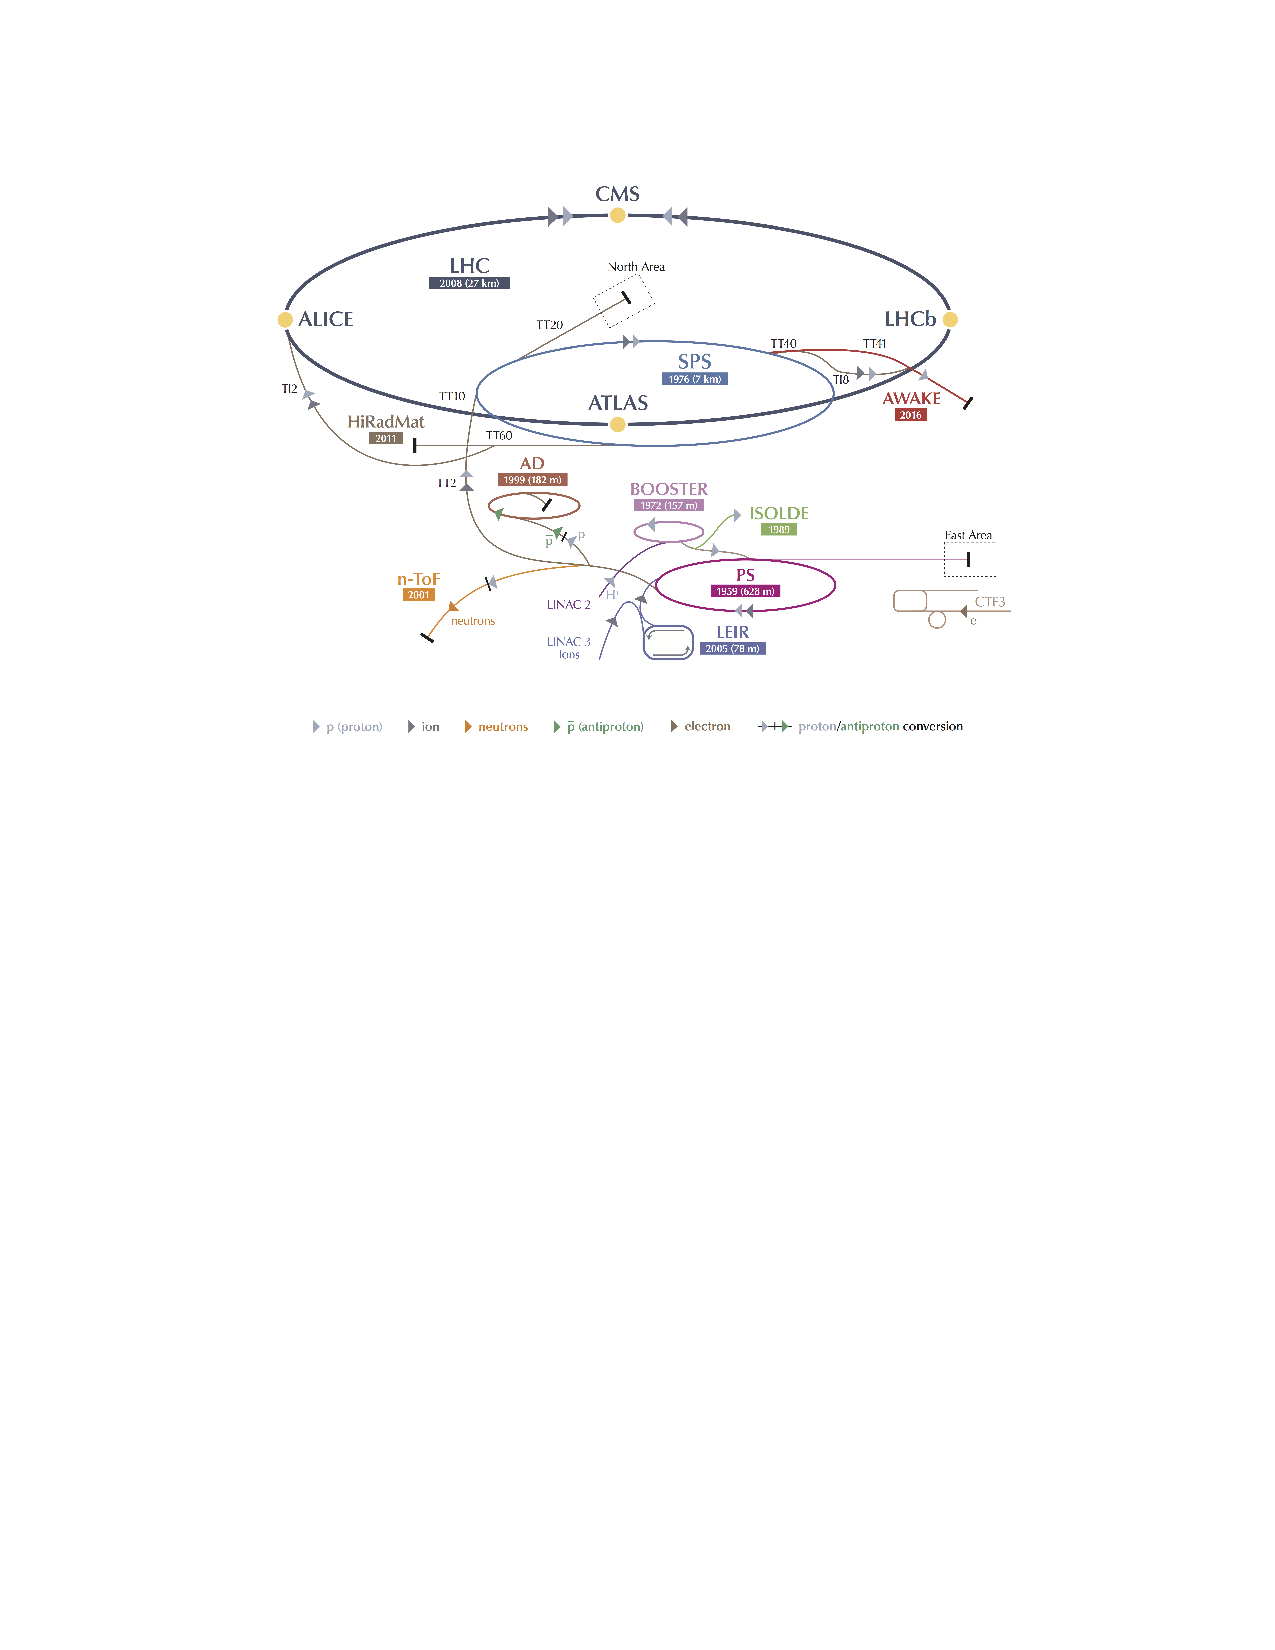
\includegraphics[width=0.9\textwidth]{figures/lhc_protons.pdf}
\caption{Schematic of the CERN accelerator complex.}
\label{fig:lhc}
\end{figure}


\section{The CMS detector}

CMS was designed with the following requirements in mind (in no particular order):
\begin{itemize}
\item Good muon identification and momentum resolution over a wide range of momenta and
angles, good dimuon mass resolution (1\% at 100 GeV), and the ability to determine unambiguously
the charge of muons with p < 1 TeV
\item Good charged-particle momentum resolution and reconstruction efficiency in the inner
tracker. Efficient triggering and offline tagging of $\tau$'s and b-jets, requiring pixel detectors
close to the interaction region
\item Good electromagnetic energy resolution, good diphoton and dielectron mass resolution (1\% at 100 GeV),
wide geometric coverage, ${\pi}^{0}$ meson rejection, and efficient photon and lepton
isolation at high luminosities
\item Good missing transverse energy and dijet mass resolution, requiring hadron calorimeters
with a large hermetic geometric coverage and with fine lateral segmentation
\end{itemize}

\begin{figure}[hb]
\centering
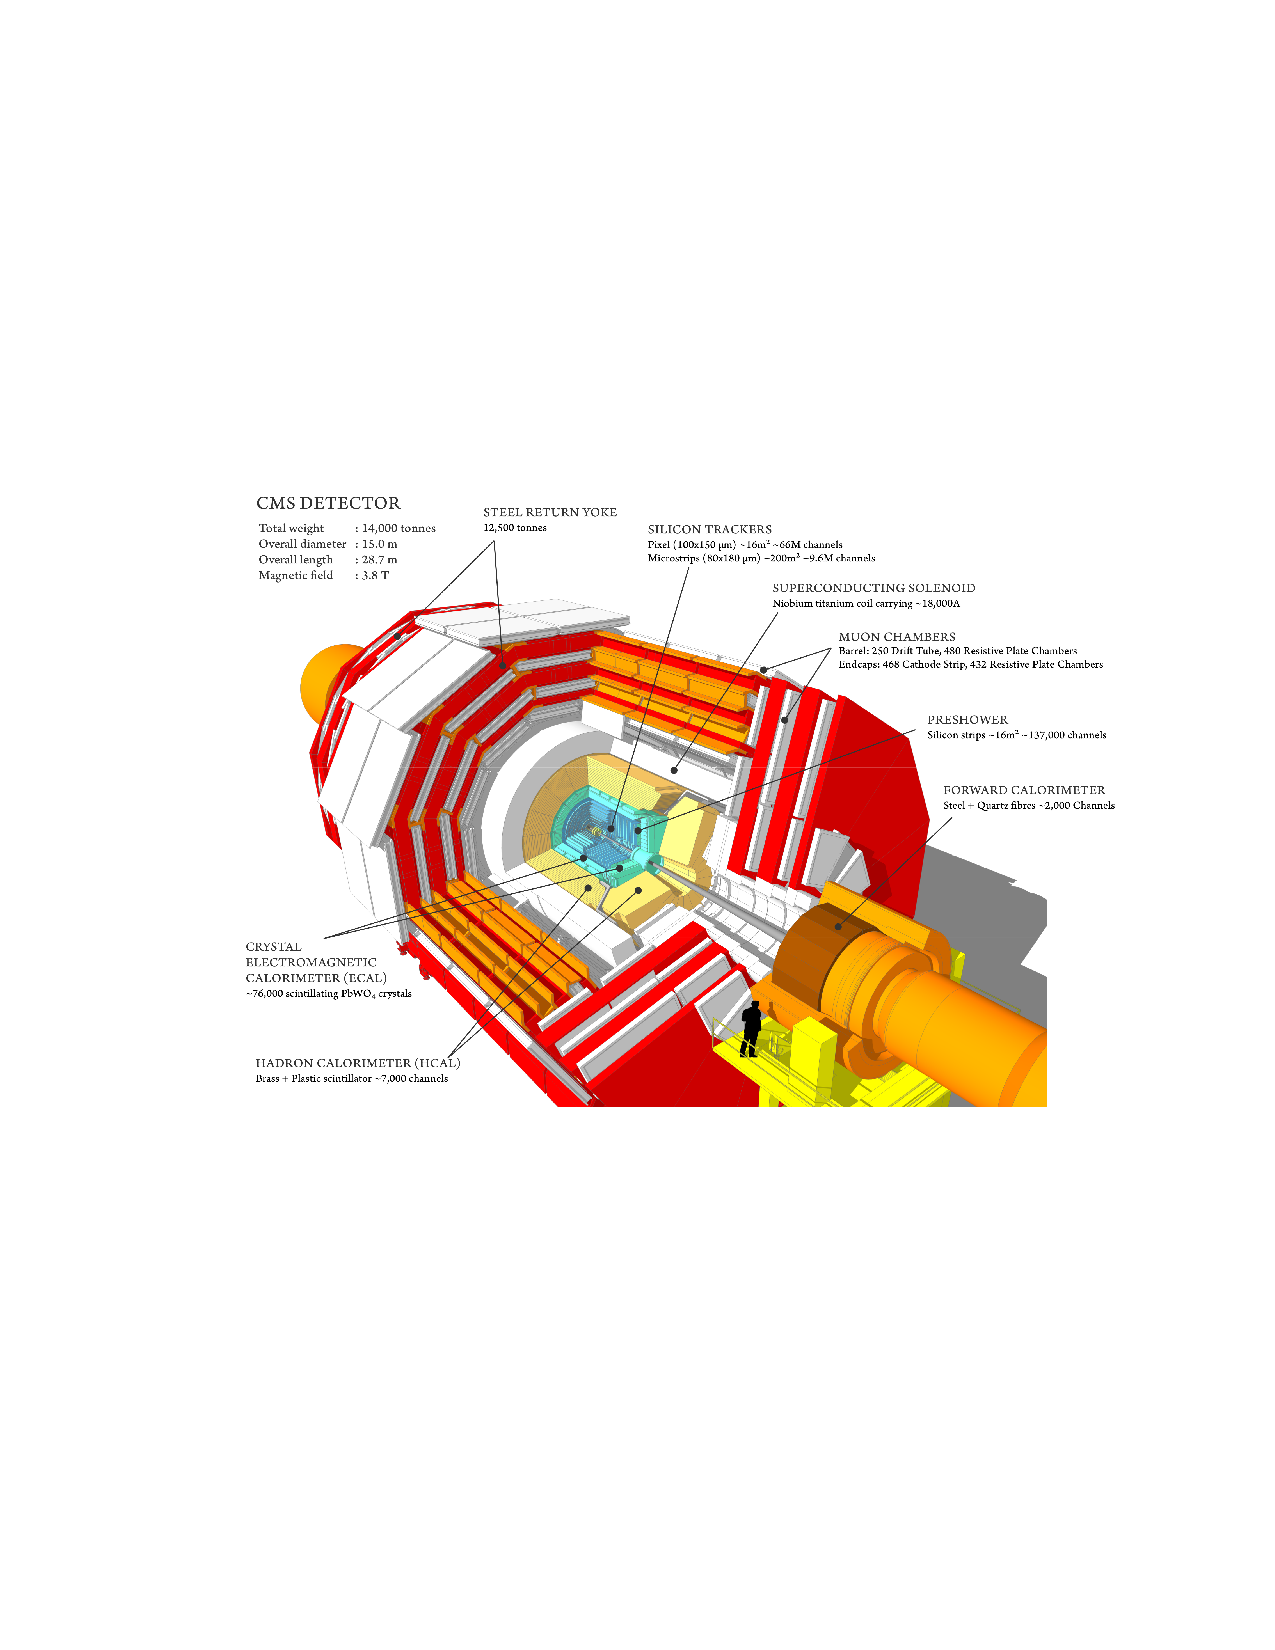
\includegraphics[width=0.95\textwidth]{figures/cms_detector.pdf}
\caption{Schematic of the CMS detector.}
\label{fig:cmsdetector}
\end{figure}

The central feature of the CMS apparatus is a superconducting solenoid of 6 m internal diameter, providing a magnetic field of 3.8 T.
Within the solenoid volume are a silicon pixel and strip tracker, a lead tungstate crystal electromagnetic calorimeter (ECAL), and a brass and scintillator hadron calorimeter (HCAL), each composed of a barrel and two endcap sections. 
Forward calorimeters extend the pseudorapidity coverage provided by the barrel and endcap detectors. 
Muons are detected in gas-ionization chambers embedded in the steel flux-return yoke outside the solenoid.

Events of interest are selected using a two-tiered trigger system~\cite{Khachatryan:2016bia}.
The first level, composed of custom hardware processors, uses information from the calorimeters and muon detectors to select events at a rate of around 100 kHz within a time interval of less than 4 $\mu$s.
The second level, known as the high-level trigger, consists of a farm of processors running a version of the full event reconstruction software optimized for fast processing, and reduces the event rate to around 1 kHz before data storage.

\subsubsection{Coordinate system}
To describe location, CMS uses a standard right-handed Cartesian coordinate system where 
the $x$ direction points to the center of the LHC ring, 
the $y$ direction points to the sky,
and the $z$ direction points in the counterclockwise beam direction at the interaction point.
This is used for locating interaction vertices and tracks' impact parameters with respect to those vertices.
However, this work will also frequently use a set of modified spherical coordinates $(r,\phi,\eta)$
which are conventional in particle physics.
Here, $r$ is the radial coordinate, $\phi$ is the azimuthal angle, and $\eta$ is the \textit{pseudorapidity}, given by
\begin{equation}
\eta  \equiv {-} \mathrm{ln}\:\mathrm{tan}\:\frac{\theta}{2} \implies \theta \equiv 2\:\mathrm{arctan} \left(e^{-\eta}\right)
\label{eq:eta}
\end{equation}
where $\theta$ is the polar angle. 
In these coordinates, the transverse momentum $p_T$ of a particle is related to its total momentum $|\vec{p}|$ and the hyperbolic secant of pseudorapidity as
\begin{equation}
p_T = |\vec{p}|~\mathrm{sech}~\eta
\end{equation}

A variable used to denote the angular separation between two objects in the detector is $\Delta R$,
which is defined as
\begin{equation}
\Delta R = \sqrt{(\phi_1-\phi_2)^2 + (\eta_1-\eta_2)^2}
\end{equation}

\subsection{Trackers}

The inner tracking system of CMS is designed to provide a precise and efficient measurement
of the trajectories of charged particles emerging from the LHC collisions, as well as a precise
reconstruction of secondary vertices. It surrounds the interaction point and has a length of 5.8 m
and a diameter of 2.5 m. The CMS solenoid provides a homogeneous magnetic field of 4 T over
the full volume of the tracker.

At the LHC design luminosity of 1034 cm\textsuperscript{-2} s\textsuperscript{-1},
there are on average about 1000 particles from more than 20 overlapping proton-proton interactions traversing
the tracker for each bunch crossing, i.e. every 25 ns. Therefore, a detector technology featuring high
granularity and fast response is required, such that the trajectories can be identified reliably and
attributed to the correct bunch crossing. However, these features imply a high power density of
the on-detector electronics which in turn requires efficient cooling. This is in direct conflict with
the aim of keeping to the minimum the amount of material in order to limit multiple scattering,
bremsstrahlung, photon conversion, and nuclear interactions. Thus, the design was optimized to balance these competing needs.

The intense particle flux will also cause severe radiation damage to the tracking system.
The main challenge in the design of the tracking system was to develop detector components able
to operate in this harsh environment for an expected lifetime of 10 years. These requirements on
granularity, speed and radiation hardness lead to a tracker design entirely based on silicon detector
technology. The CMS tracker is composed of a pixel detector with three barrel layers at radii
between 4.4 cm and 10.2 cm and a silicon strip tracker with 10 barrel detection layers extending
outwards to a radius of 1.1 m. Each system is completed by endcaps which consist of 2 disks in
the pixel detector and 3 plus 9 disks in the strip tracker on each side of the barrel, extending the
acceptance of the tracker up to a pseudorapidity of $|\eta| < 2.5$. With about 200 m\textsuperscript{2} of active silicon
area the CMS tracker is the largest silicon tracker ever built.

\begin{figure}[hbtp]
\centering
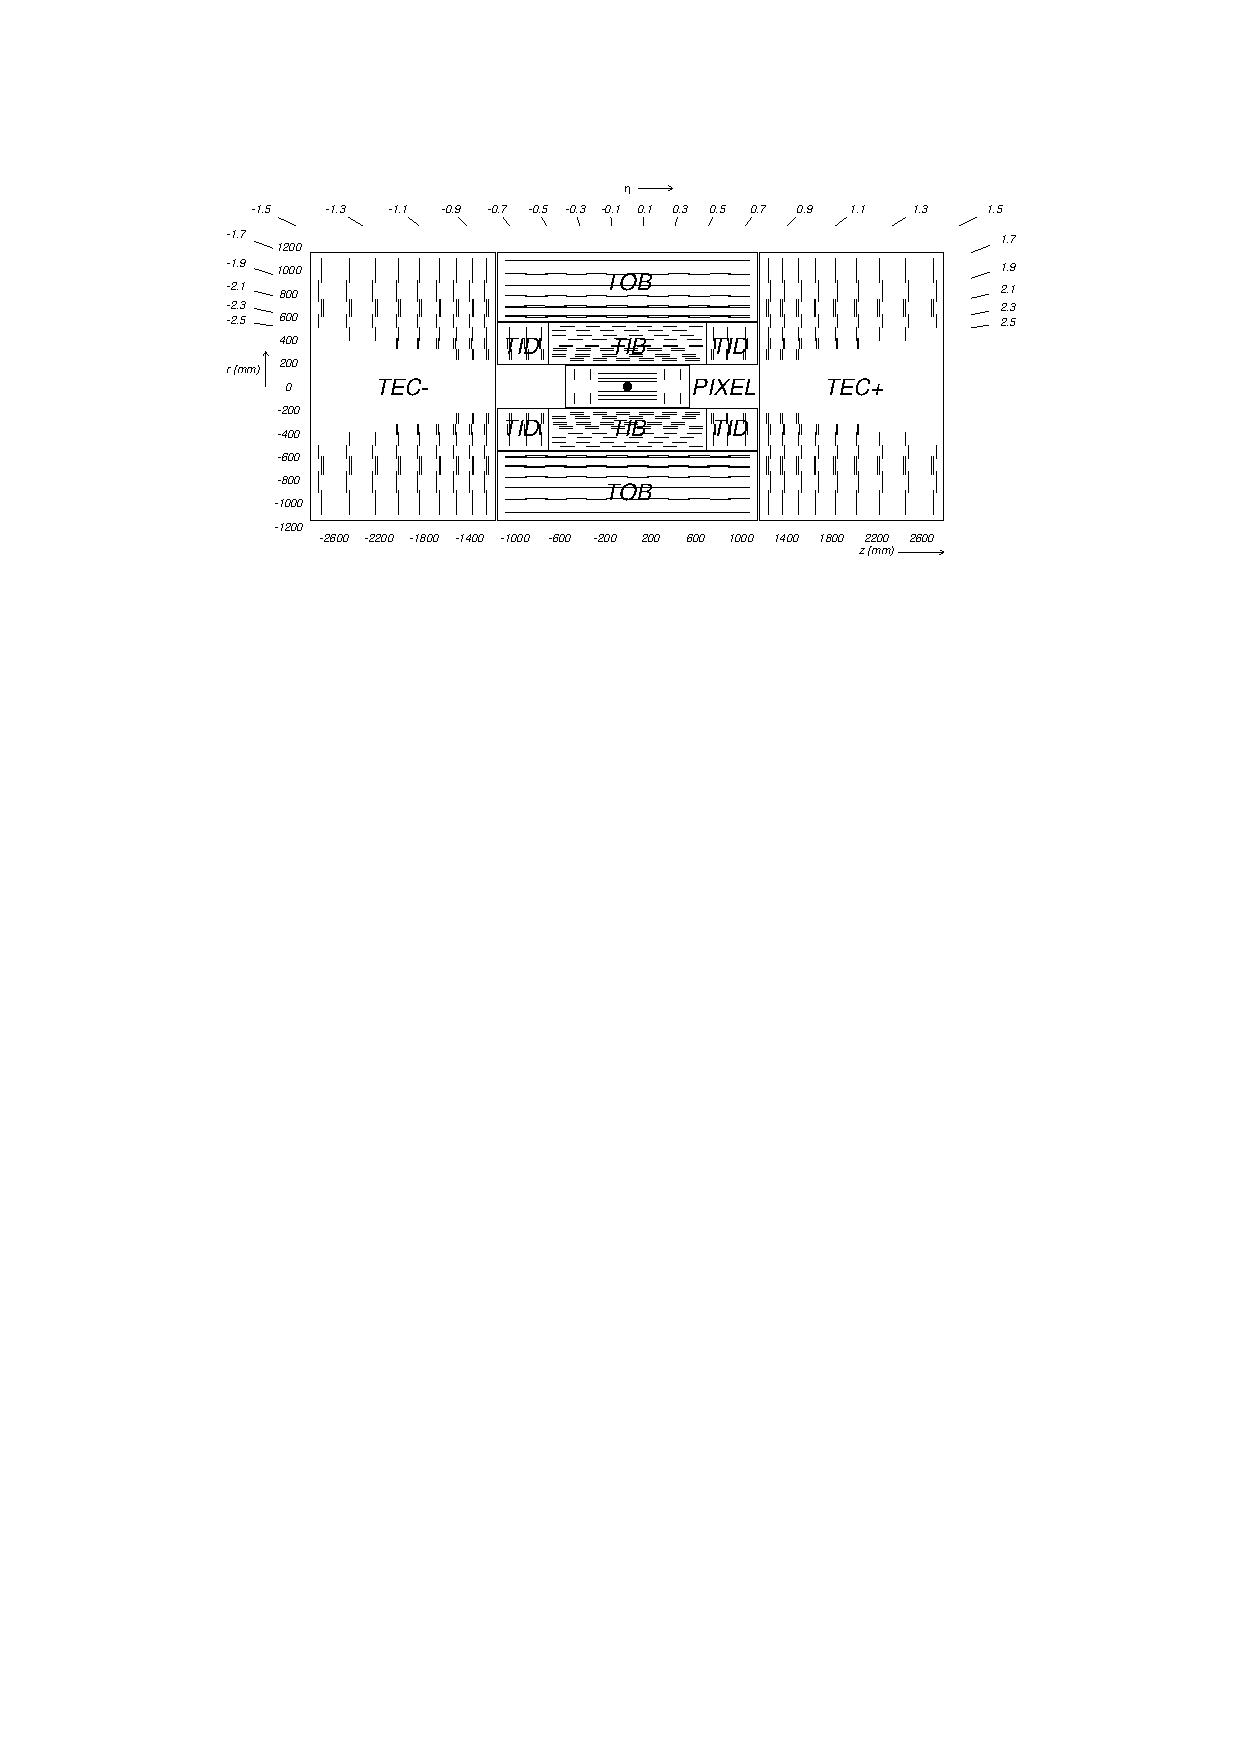
\includegraphics[width=0.9\textwidth]{figures/cms_tracker.pdf}
\caption{Layout of the CMS tracker. From \cite{Chatrchyan:2008aa}.}
\label{fig:cms_tracker}
\end{figure}

\subsection{Electromagnetic calorimeter}
The electromagnetic calorimeter of CMS (ECAL) is a hermetic homogeneous calorimeter made of
61,200 lead tungstate ($\textrm{PbWO}_{\textrm{4}}$) crystals mounted in the central barrel part,
and 7,324 crystals in each of the two endcaps. 
A preshower detector is placed in front of the endcap crystals.
Avalanche photodiodes (APDs) are used as photodetectors in the barrel and vacuum phototriodes
(VPTs) in the endcaps. The use of high density crystals has allowed the design of a calorimeter
which is fast, has fine granularity and is radiation resistant, all important characteristics in the LHC
environment. 
One of the driving criteria in the design was the capability to detect the decay to two
photons of the postulated Higgs boson.
This capability is enhanced by the good energy resolution
provided by a homogeneous crystal calorimeter.

\begin{figure}
\centering
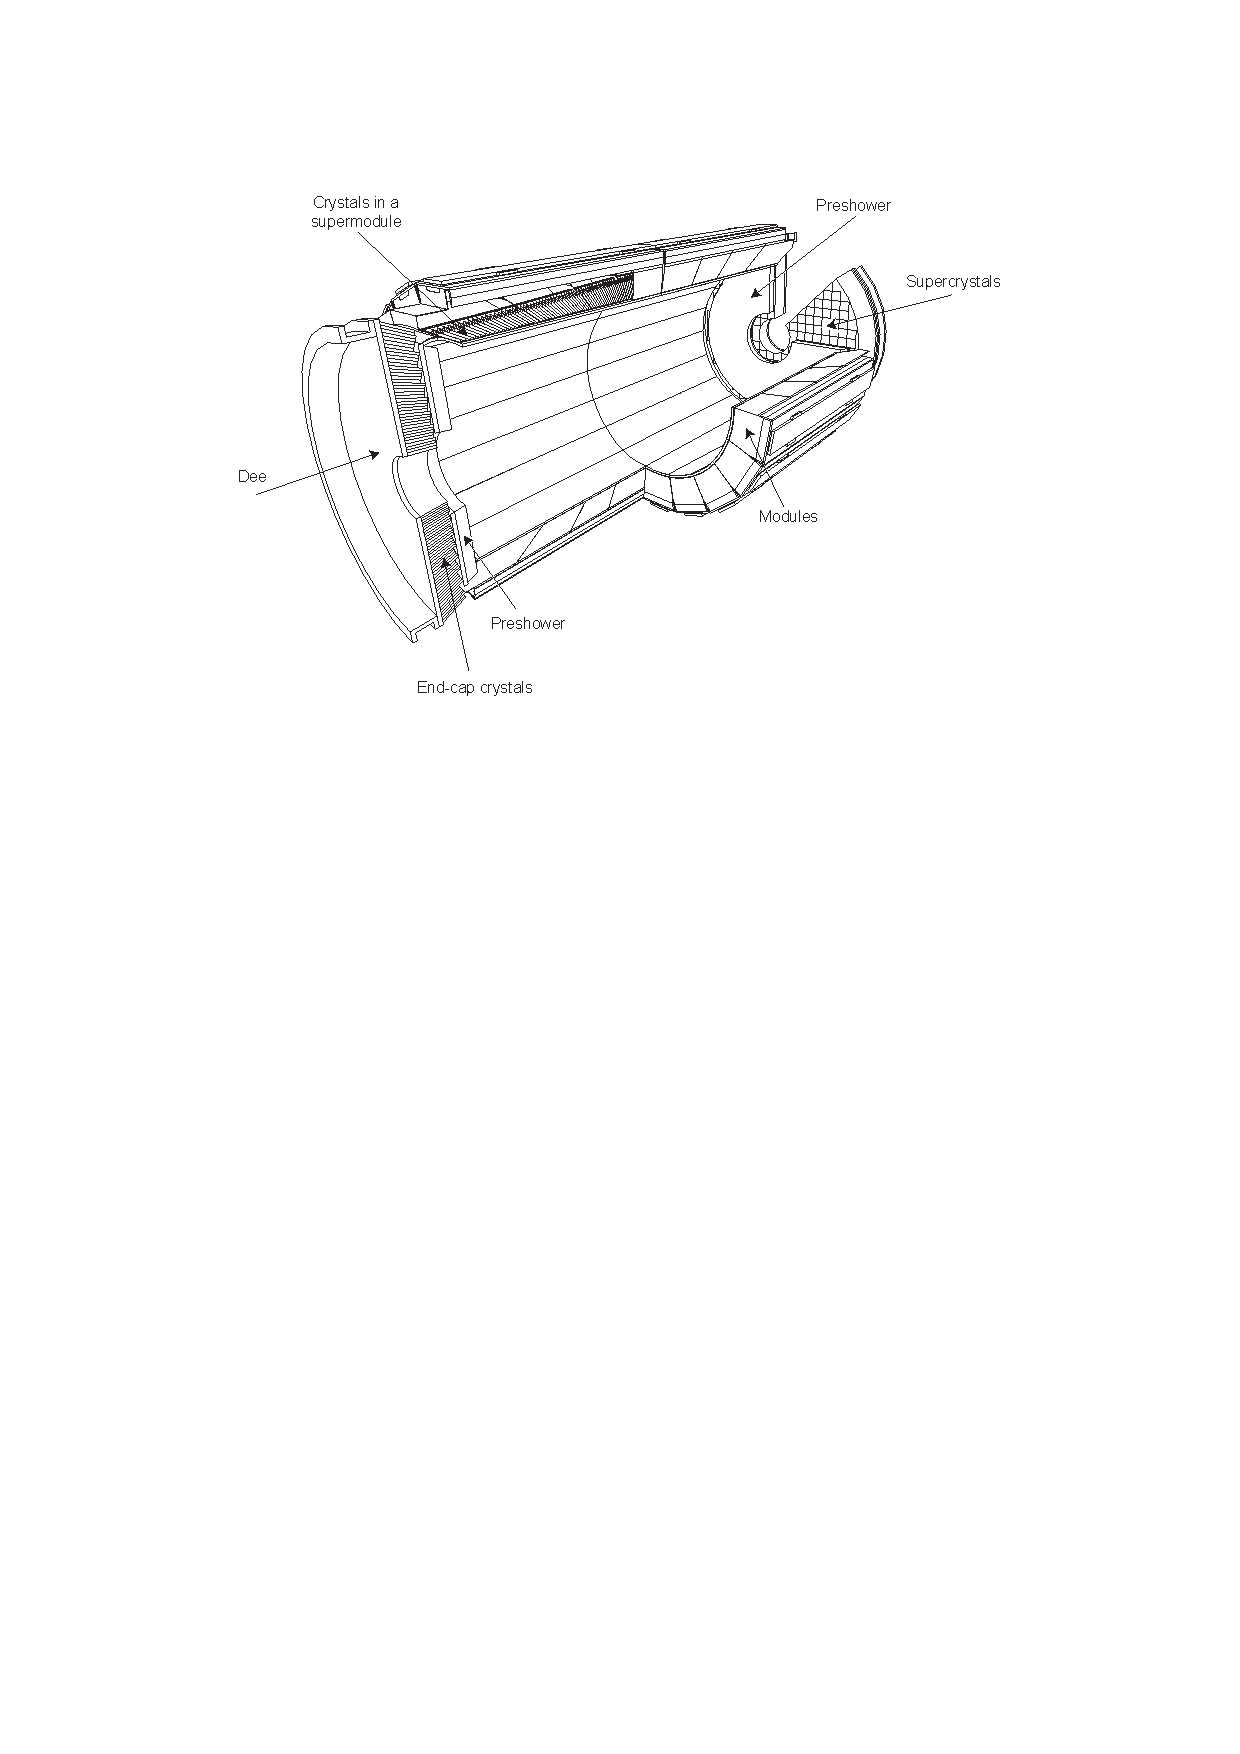
\includegraphics[width=0.9\textwidth]{figures/ecal_layout.pdf}
\caption{Layout of the CMS electromagnetic calorimeter showing the arrangement of crystal
modules, supermodules and endcaps, with the preshower in front. From \cite{Chatrchyan:2008aa}.}
\label{fig:ecal_layout}
\end{figure}

The number of scintillation photons and the electronic amplification thereof both are decreasing with temperature. 
So the ECAL must be kept at a stable temperature of $18\pm0.05$\textdegree~ C.
Water cooling and aluminum tubing are used to meet this need.

\subsubsection{ECAL barrel}
The ECAL barrel (EB) covers the pseudorapidity range $|\eta|<1.479$.
The granularity is 360 in $\phi$ and 170 in $\eta$, giving 61,200 crystals in all.
The crystals have a tapered shape.
They are mounted in a quasi-projective geometry to avoid cracks aligned with particle trajectories.
In other words, their central axes are not exactly parallel to a path from the interaction point, 
in either the $\phi$ or $\eta$ projections.
The crystal cross-section corresponds to approximately $0.0174 \times 0.0174$ in $\eta\times\phi$
or $22 \times 22$ mm\textsuperscript{2} at the front face of the crystal--and $26 \times 26$ mm\textsuperscript{2}
at the rear face.
The crystals' radial length is 230 mm, corresponding to 25.8 radiation lengths.

\begin{figure}
\centering
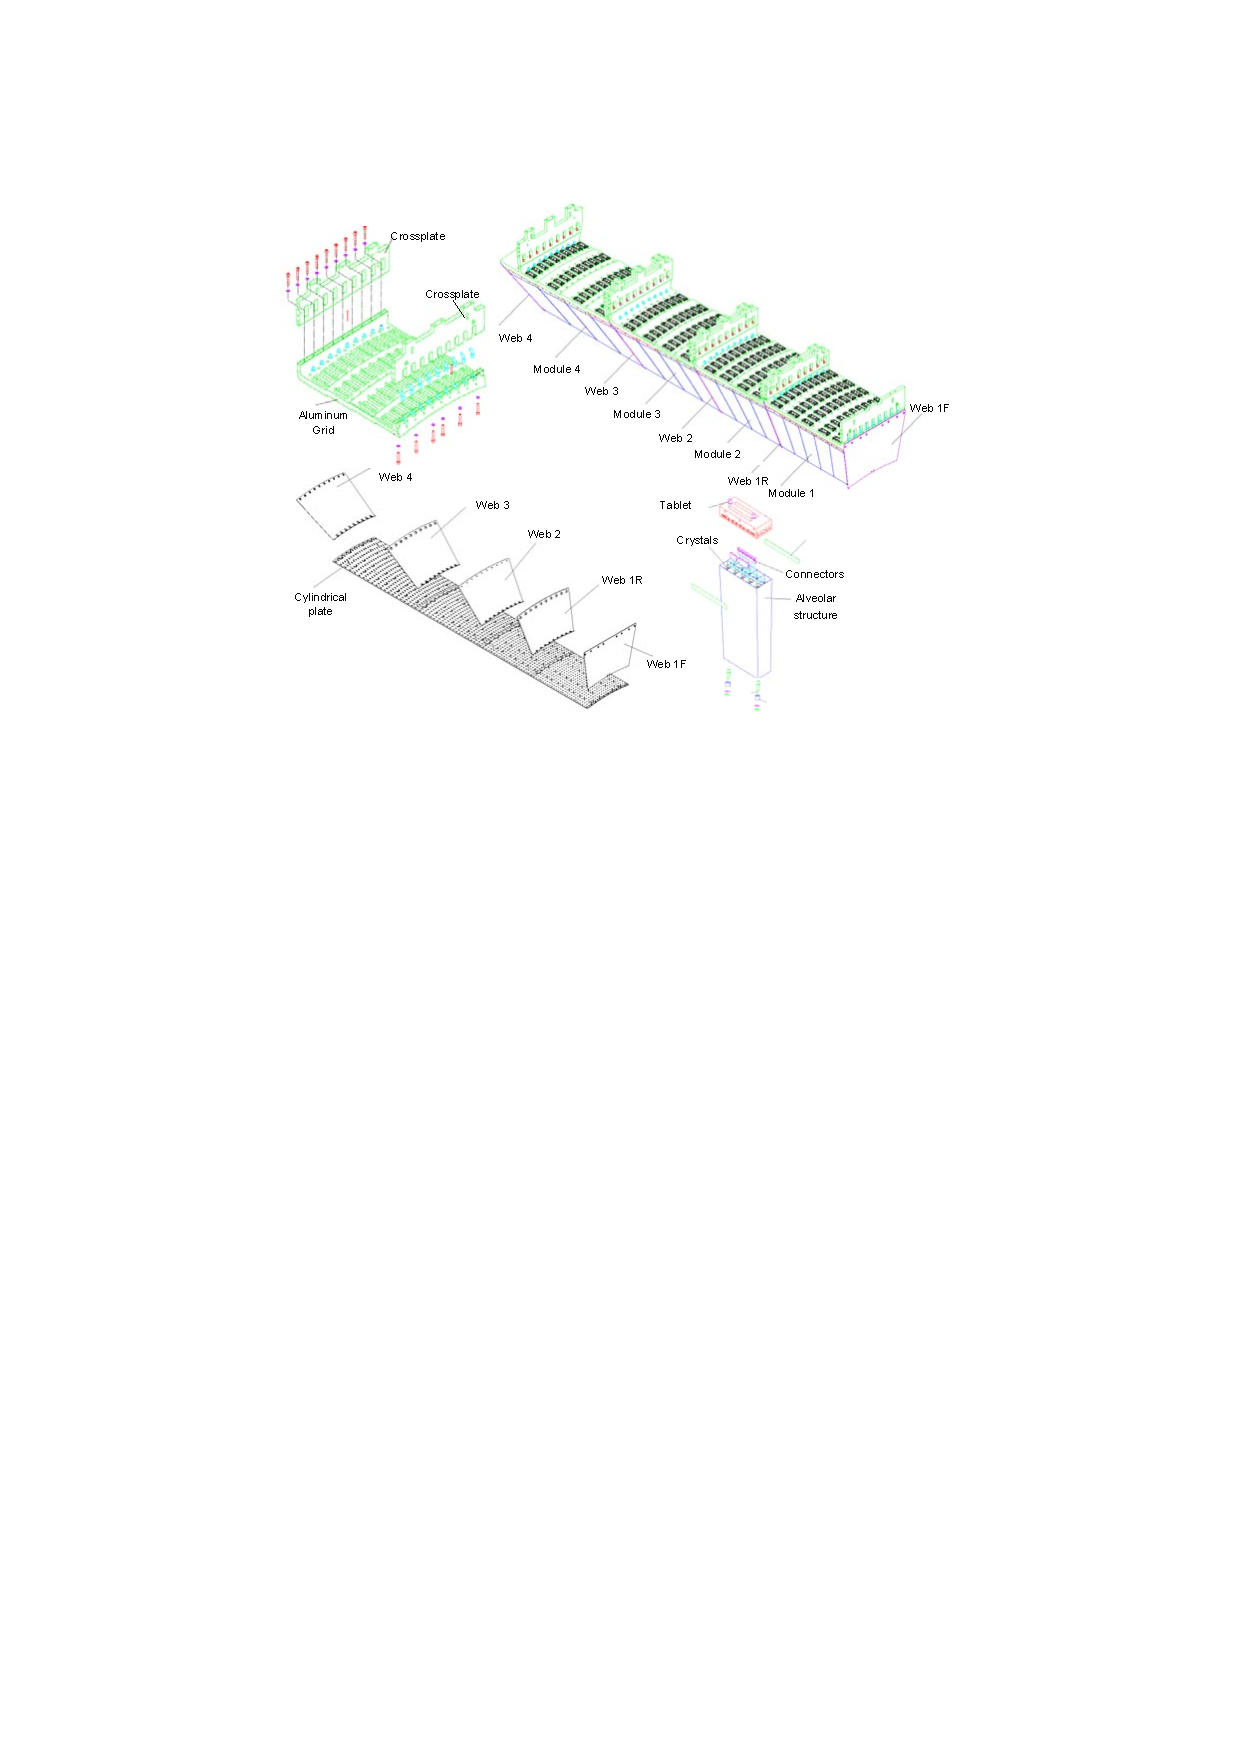
\includegraphics[width=0.9\textwidth]{figures/ecal_barrel.pdf}
\caption{Layout of the ECAL barrel. From \cite{Chatrchyan:2008aa}.}
\label{fig:ecal_barrel}
\end{figure}

In the barrel, the scintillation photons are collected by Hamamatsu type S8148 reverse structure avalanche photodiodes.
Their active area is $5\times5$ mm\textsuperscript{2}. Two are mounted on each crystal.

\subsubsection{ECAL endcaps}
The ECAL endcaps (EE) cover the rapidity range $1.479 < \eta < 2.5$.
The distance from the interaction point and the endcaps is 315.4 cm with the 4 T magnetic field on.
Most of each endcap consists of identically shaped crystals grouped in mechanical units of $5\times5$ crystals, called supercrystals.
As with the EB crystals, the central axes of the EE supercrystals are not exactly parallel to a path from the interaction point. 
The front face of these crystals has an area of $28.62\times28.62$ mm\textsuperscript{2}.
The rear face has an area of $30\times30$ mm\textsuperscript{2}.
The crystals' length is 220 mm or 24.7 radiation lengths.

In the endcaps, the scintillation photons are collected by type PMT188 vacuum phototriodes
from National Research Institute Electron in St. Petersburg.
Their active area is 280 mm\textsuperscript{2}. One is mounted on each crystal.

It is relevant to make a note here that the physical cracks between the EB and EEs exist at $1.4442 < |\eta| < 1.566$. 
This has a negative effect on the electron identification efficiency, to be described in great detail later.
This motivates the non-intuitive kinematic binnings in $\eta$ which are used later
in Chapter~\ref{chap:efficiency} and Appendix~\ref{app:efficiency}.

\subsection{Hadron calorimeters}
The hadron calorimeters (HCALs) exist to measure the energy of hadrons and hadronic jets.
Most hadrons pass through the ECAL due to its limited stopping power and then deposit the rest of their energy in the HCAL.
Muons, and the few energetic hadrons which punch through the HCAL, traverse past it and reach the muon system.
From the visible particle energies recorded in the ECAL, HCAL, and muon systems, 
it is possible to construct the quantity of missing transverse energy in order to
infer the production of neutrinos or exotic particles.
Figure~\ref{fig:hcalslice} shows the longitudinal view of the CMS detector. The dashed lines are at fixed $\eta$ values. 
The hadron calorimeter barrel and endcaps sit behind the tracker and the electromagnetic
calorimeter as seen from the interaction point. The hadron calorimeter barrel is radially restricted
between the outer extent of the electromagnetic calorimeter (R = 1.77 m) and the inner extent of
the magnet coil (R = 2.95 m). This constrains the total amount of material which can be put in
to absorb the hadronic shower. Therefore, an outer hadron calorimeter or tail catcher is placed
outside the solenoid complementing the barrel calorimeter. Beyond $|\eta| = 3$, the forward hadron
calorimeters placed at 11.2 m from the interaction point extend the pseudorapidity coverage down
to $|\eta| = 5.2$ using a Cherenkov-based, radiation-hard technology.
The HCAL subsystems are described briefly below, with more detailed information on the geometry and 
readout being available in~\cite{CMSTDR}.

\begin{figure}
\centering
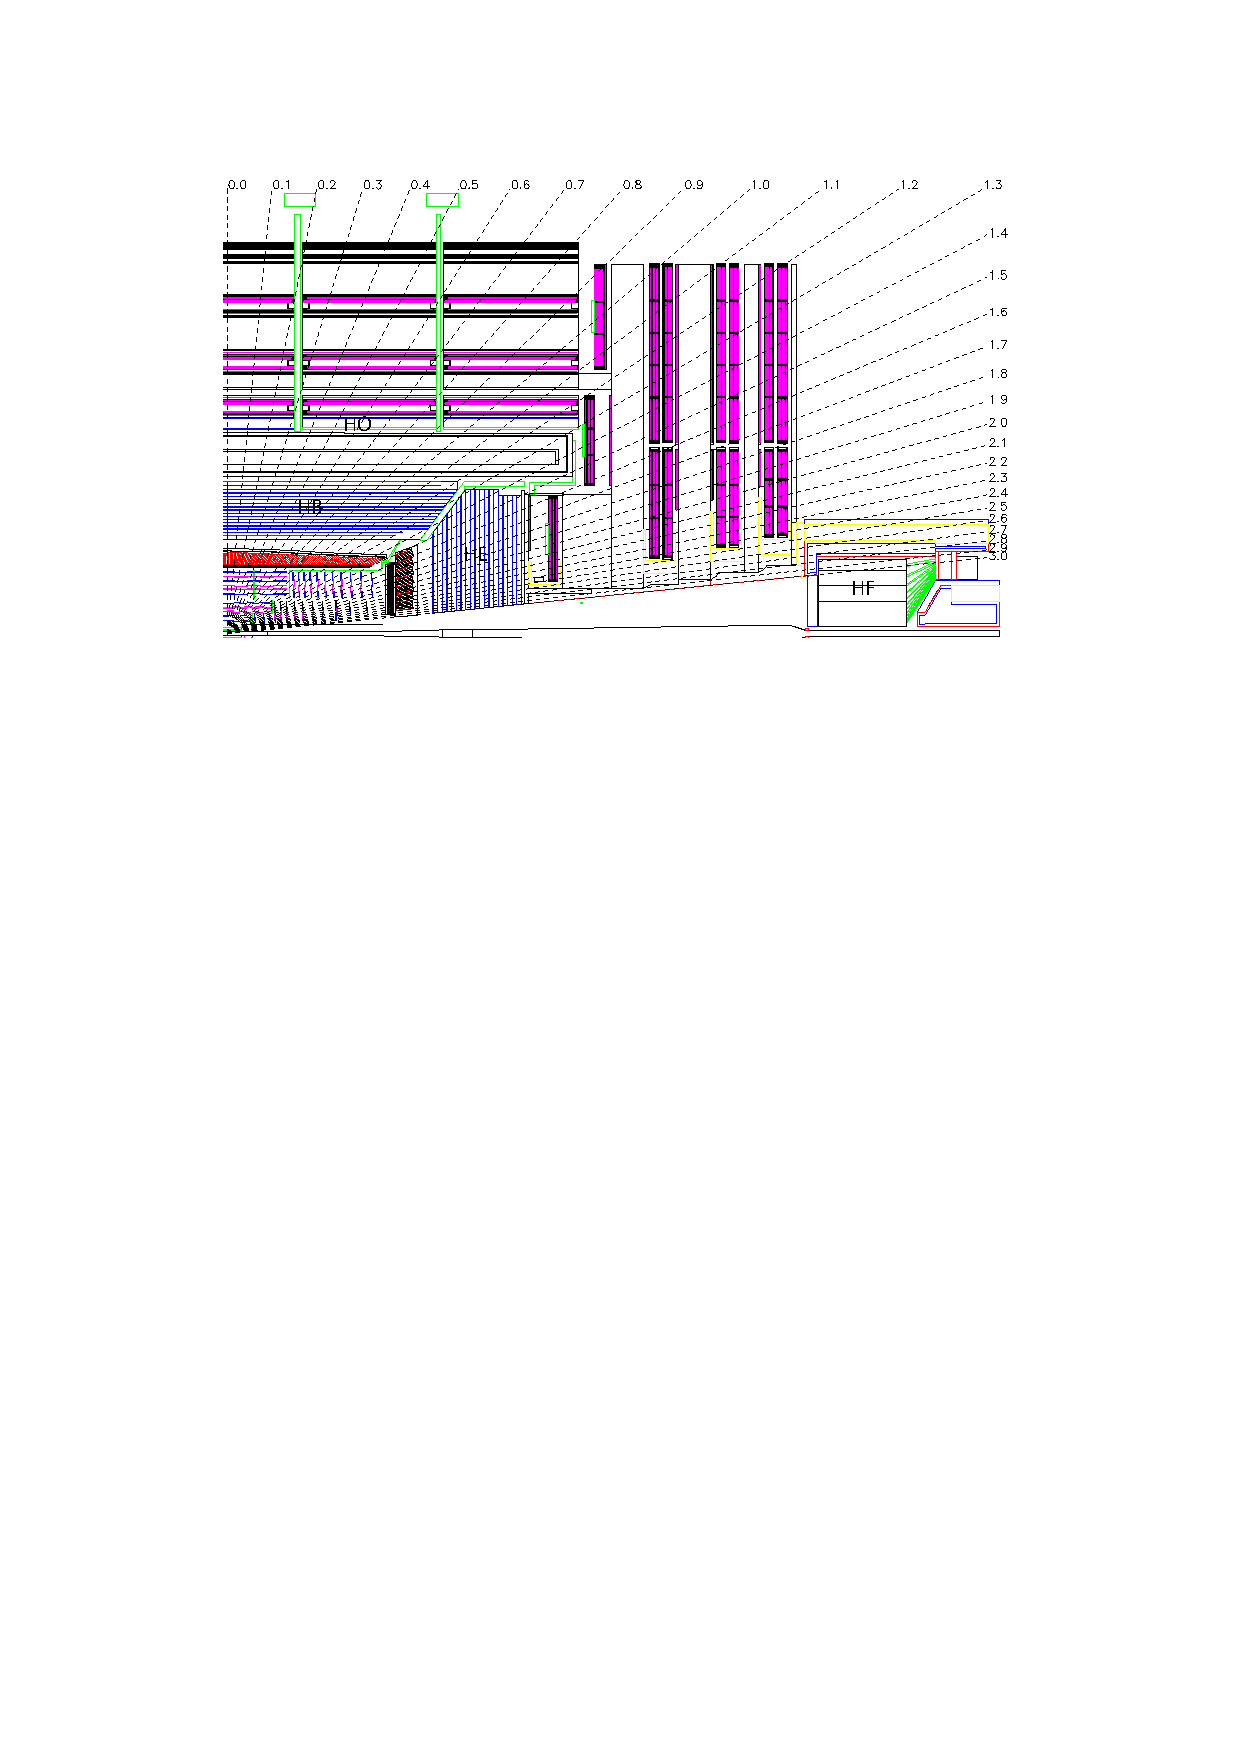
\includegraphics[width=0.98\textwidth]{figures/hcalslice.pdf}
\caption{Longitudinal slice of the CMS detector showing the locations of the hadron barrel
(HB), endcap (HE), outer (HO) and forward (HF) calorimeters.}
\label{fig:hcalslice}
\end{figure}

\subsubsection{HCAL barrel}
The HCAL barrel (HB) is a sampling calorimeter and covers the pseudorapidity range $|\eta| < 1.3$.
It consists of 36 identical azimuthal wedges which form two half-barrels. 
The wedges are constructed out of flat brass absorber plates which are parallel
to the beam axis.  Each wedge is segmented into four azimuthal angle ($\phi$) sectors. 
The innermost and outermost plates are made of stainless steel for structural strength.

The absorber consists of a front steel plate 40 mm thick,
followed by eight 50.5 mm thick brass plates, six 56.5 mm thick brass plates,
and a 75 mm thick steel back plate.
The last layer is thicker to correct for late developing showers which could leak out the back.
The total absorber thickness at 90\textdegree~is 5.82 interaction lengths ($\lambda_I$).
The HB effective thickness increases with polar angle ($\theta$) as $1/\textrm{sin}\:\theta$,
resulting in 10.6 $\lambda_I$ at $|\eta| = 1.3$. 

The HB baseline active material is 3.7 mm thick Kuraray SCSN81 plastic scintillator, 
chosen for its long-term stability and moderate radiation hardness. 
The first layer of scintillator is located in front of the steel support plate, 
and is made of 9 mm thick Bicron BC408. 
Its purpose is to sample hadronic showers developing in the inert material between
the ECAL barrel and the HCAL barrel.
The plastic scintillator is divided into 16 $\eta$ sectors, resulting in a segmentation of $(\Delta\eta, \Delta\phi) = (0.087, 0.087)$. 

\subsubsection{HCAL endcaps}

The hadron calorimeter endcaps (HE) cover the rapidity range $1.3 < |\eta| < 3$. 
It is designed for high radiation tolerance, in order to survive 10 MRad after 10 years of operation.
The total length of the endcap calorimeter, after the ECAL and HCAL endcaps, is about 10 interaction lengths. 

The absorber is made of C26000 cartridge brass. The material was chosen because it is non-magnetic, has a short interaction length and was available at a relatively low cost.
The absorber is assembled in a staggered geometry which minimizes the cracks between HB and HE and contains no projective dead material. 

The scintillators are of trapezoidal shape and there are 18 layers of them in total. 
The first layer are made of 9 mm thick Bicron BC408. All the rest are made of 3.7 mm thick SCSN81.
The scintillation light is read out via wavelength shifting fibers. 
The granularity of the calorimeters is $(\Delta\eta, \Delta\phi) = (0.087, 0.087)$ for $|\eta| < 1.6$ and $(\Delta\eta, \Delta\phi) = (0.170, 0.170)$ for $|\eta| \geq 1.6$.

\subsubsection{HCAL outer}
The combined stopping power of the ECAL and HCAL barrels does not provide adequate stopping
power in the central region $|\eta| < 1.3$. This is problematic for the missing energy resolution.
To further measure and contain these showers, the hadron calorimeter is extended outside the solenoid with a tail catcher called the HO. Only 40 mm of space in the radial direction is available, 
24 mm of which is used for aluminum honeycomb support structures.

The scintillator plates of the HO are made of 10 mm thick Bicron BC408. There are 5 rings in $\eta$, each of those rings having 12 identical $\phi$ sectors, and each of those sectors having 6 azimuthal slices.
The sizes and positions of the tiles in HO are supposed to roughly map the layers of HB
to make towers of granularity $(\Delta\eta, \Delta\phi) = (0.087, 0.087)$.

The magnetic solenoid coil is used as an additional absorber equal to $1.4/\textrm{sin}\:\theta$ interaction lengths.
Outside the vacuum tank, the magnetic field is returned through an iron yoke roughly 20 mm thick, with 5 rings corresponding to the scintillator plates.
The central ring has scintillators both inside and outside of the iron yoke ring.
The others have scintillators only outside their yoke rings.
All told, the total depth of the calorimeter system is extended to a minimum of
$11.8\:\lambda_I$ except at the barrel-endcap boundary region at around $|\eta|=1.4$.

\subsubsection{HCAL forward}
The forward calorimeter, or HF, exists in an extremely hostile environment. 
At $|\eta|=5$ we expect to have delivered 10 MGy after 10 years of operation.
The active material is fused-silica core, polymer hard-cladded quartz fibers, which have sufficient radiation hardness.
These fibers measure 600 $\pm$ \SI{10}{\micro\meter} in diameter for the fused-silica core,
$ {630}^{+5}_{-10}$ \SI{}{\micro\meter} with the polymer hard-cladding, 
and 800 $\pm$ \SI{30}{\micro\meter} with the protective acrylate buffer.

The geometry consists of a steel absorber structure composed of 5 mm thick grooved
plates. Fibers are inserted in these grooves.
The detector is functionally subdivided into two longitudinal segments. 
Half of the fibers run over the full depth of the absorber (165 cm $\approx 10\:\lambda_I$)
while the other half starts at a depth of 22 cm from the front of the detector.
These two sets of fibers are read out separately. 
This arrangement makes it possible to distinguish showers generated by electrons and photons,
which deposit the majority of their energy in the first 22 cm,
from those generated by hadrons, which produce nearly equal signals in both calorimeter segments on average. 
The absorber has grooves which make a square grid separated by 5.0 $\pm$ 0.1 mm center-to-center, with long and short fibers alternating in the grooves. 

This calorimeter is mostly sensitive to the electromagnetic component of hadronic showers.
Only light that hits the core-cladding interface at an angle larger than the critical angle (71\textdegree) contributes to the calorimeter signal in the form of Cherenkov light. 
After the quoted 10 MGy dose has accumulated over the HF lifetime, the optical transmission of the fibers is reduced just by a factor of 2.

\subsection{Muon system}
\label{ss:muonsystem}
The CMS muon system is capable of reconstructing the momentum and charge of muons over the entire
kinematic range of the LHC. 
Due to the shape of the CMS solenoid magnet, the muon system has a barrel section and 2 endcap sections.
Three types of gaseous particle detectors are used.
Since the total area of the muon detection planes is around 25,000 $\textrm{m}^2$, the 
detectors were chosen to be inexpensive but reliable.

In the barrel region, rectangular drift tubes (DT) are used, 
since there is little neutron-induced muon background, the magnetic field is uniform,
and the real muon rate is relatively low.
In the endcap regions, there is a high muon rate, high muon background, and a
very nonuniform magnetic field, so cathode strip chambers (CSC) are used there.
The third subsystem is the resistive plate chambers (RPC). Their spatial resolution is relatively poor.
But their fast response and good time resolution are useful for the trigger.
They also help resolve ambiguity in the standalone muon reconstruction,
which only uses information from the muon system.

The DTs and CSCs are each capable of triggering on muon $p_T$ independently of the other detector subsystems.
The $p_T$ resolution of this triggering muon object is 15\% in the barrel and 25\% in the endcap.
For muon $p_T$ up to $200 \GeV$, the DTs and CSCs together can give a standalone momentum resolution of 9\%.
Approaching muon momenta of $1 \TeV$, the standalone momentum resolution is 5\%.
The muon resolution is improved when combined with the tracker information.

Lastly, an alignment system measures the relative positions of the muon detectors amidst the inner tracker to optimize the momentum resolution of muons.

\begin{figure}[hbtp]
\centering
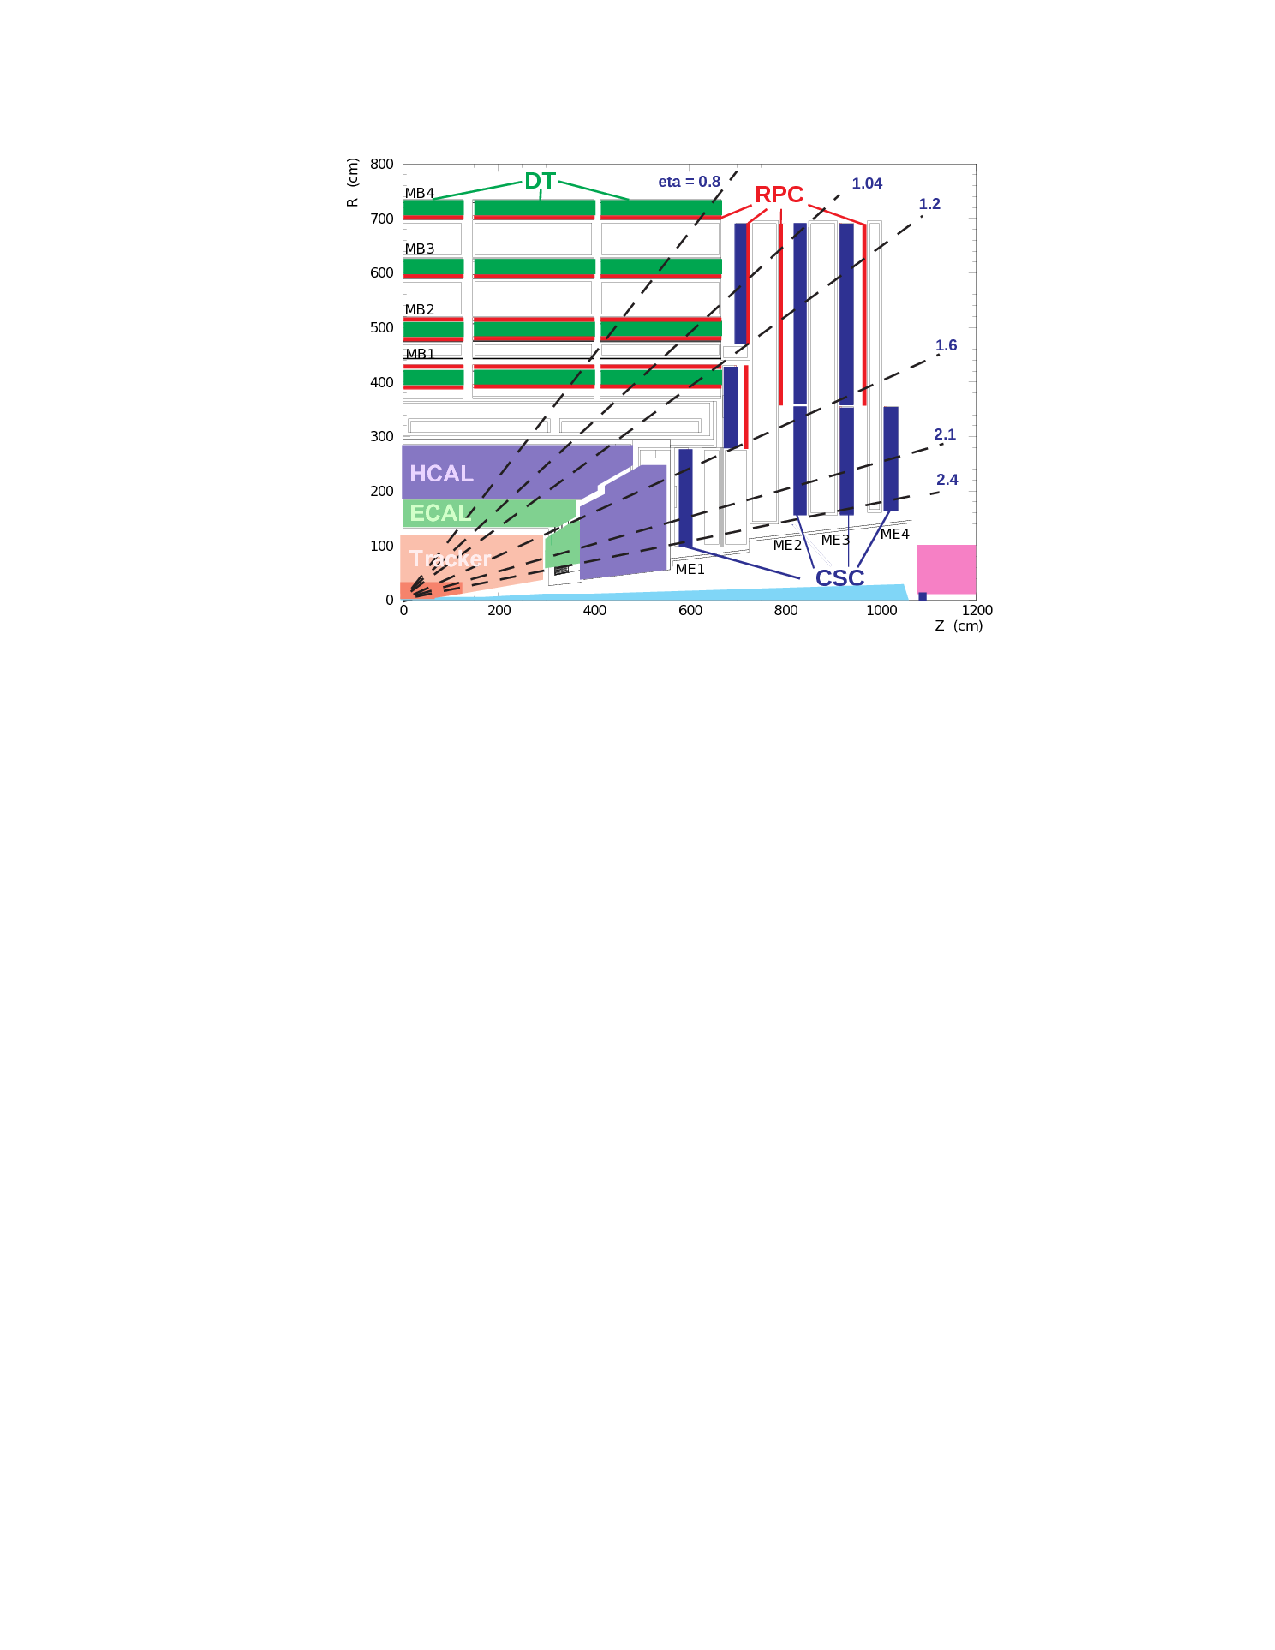
\includegraphics[width=0.8\textwidth]{figures/cms_muon_systems.pdf}
\caption{
Quarter-view of the CMS detector showing the muon system components. 
From \cite{Chatrchyan:2008aa}.
}
\label{fig:muonsystem}
\end{figure}

\subsubsection{Drift tubes}
The DTs cover the pseudorapidity region $|\eta|<1.2$.
There are 4 stations forming concentric cylinders around the beam line.
The 3 inner cylinders have 60 drift chambers each and the outer cylinder has 70.
There are about 172,000 sensitive wires of about 2.4m in length.
The maximum drift path length is 21 mm. In a gaseous admixture of 85\% Ar and 15\% $\mathrm{CO}_2$ the maximum drift time is 380 ns.
For the LHC design luminosity, this produces a negligible occupancy
and permits the use of single-hit electronics.
Meanwhile, the cell size is sufficiently large to keep the number of electronic channels low and affordable.

Each DT chamber is made of 2 or 3 superlayers (SL).
Each SL is made of layers of rectangular drift cells staggered by half a cell.
The wires in the 2 outer SLs are parallel to the beam line and provide a track measurement
in the magnetic bending plane. 
The wires in the inner SL are orthogonal to the beam line and measure the $z$ position.
This innermost SL is not present in the fourth DT station
Thus, a muon first encounters a $\phi$-measuring SL, passes through a honeycomb spacer plate,
then crosses the $z$-measuring SL and the second $\phi$-measuring SL.
Due to discontinuities in the design,
a muon could end up crossing only two stations instead of the maximum four.

One superlayer has time resolution on the order of nanoseconds.
The time measurement is delayed by the drift-time, determined by the design parameters of the drift tubes.
Using the SL information, pattern recognition circuits deliver the position and angle 
of the track segment's center of gravity with precision of 1.5 mm and 20 mrad, respectively.

\begin{figure}[hbtp]
\centering
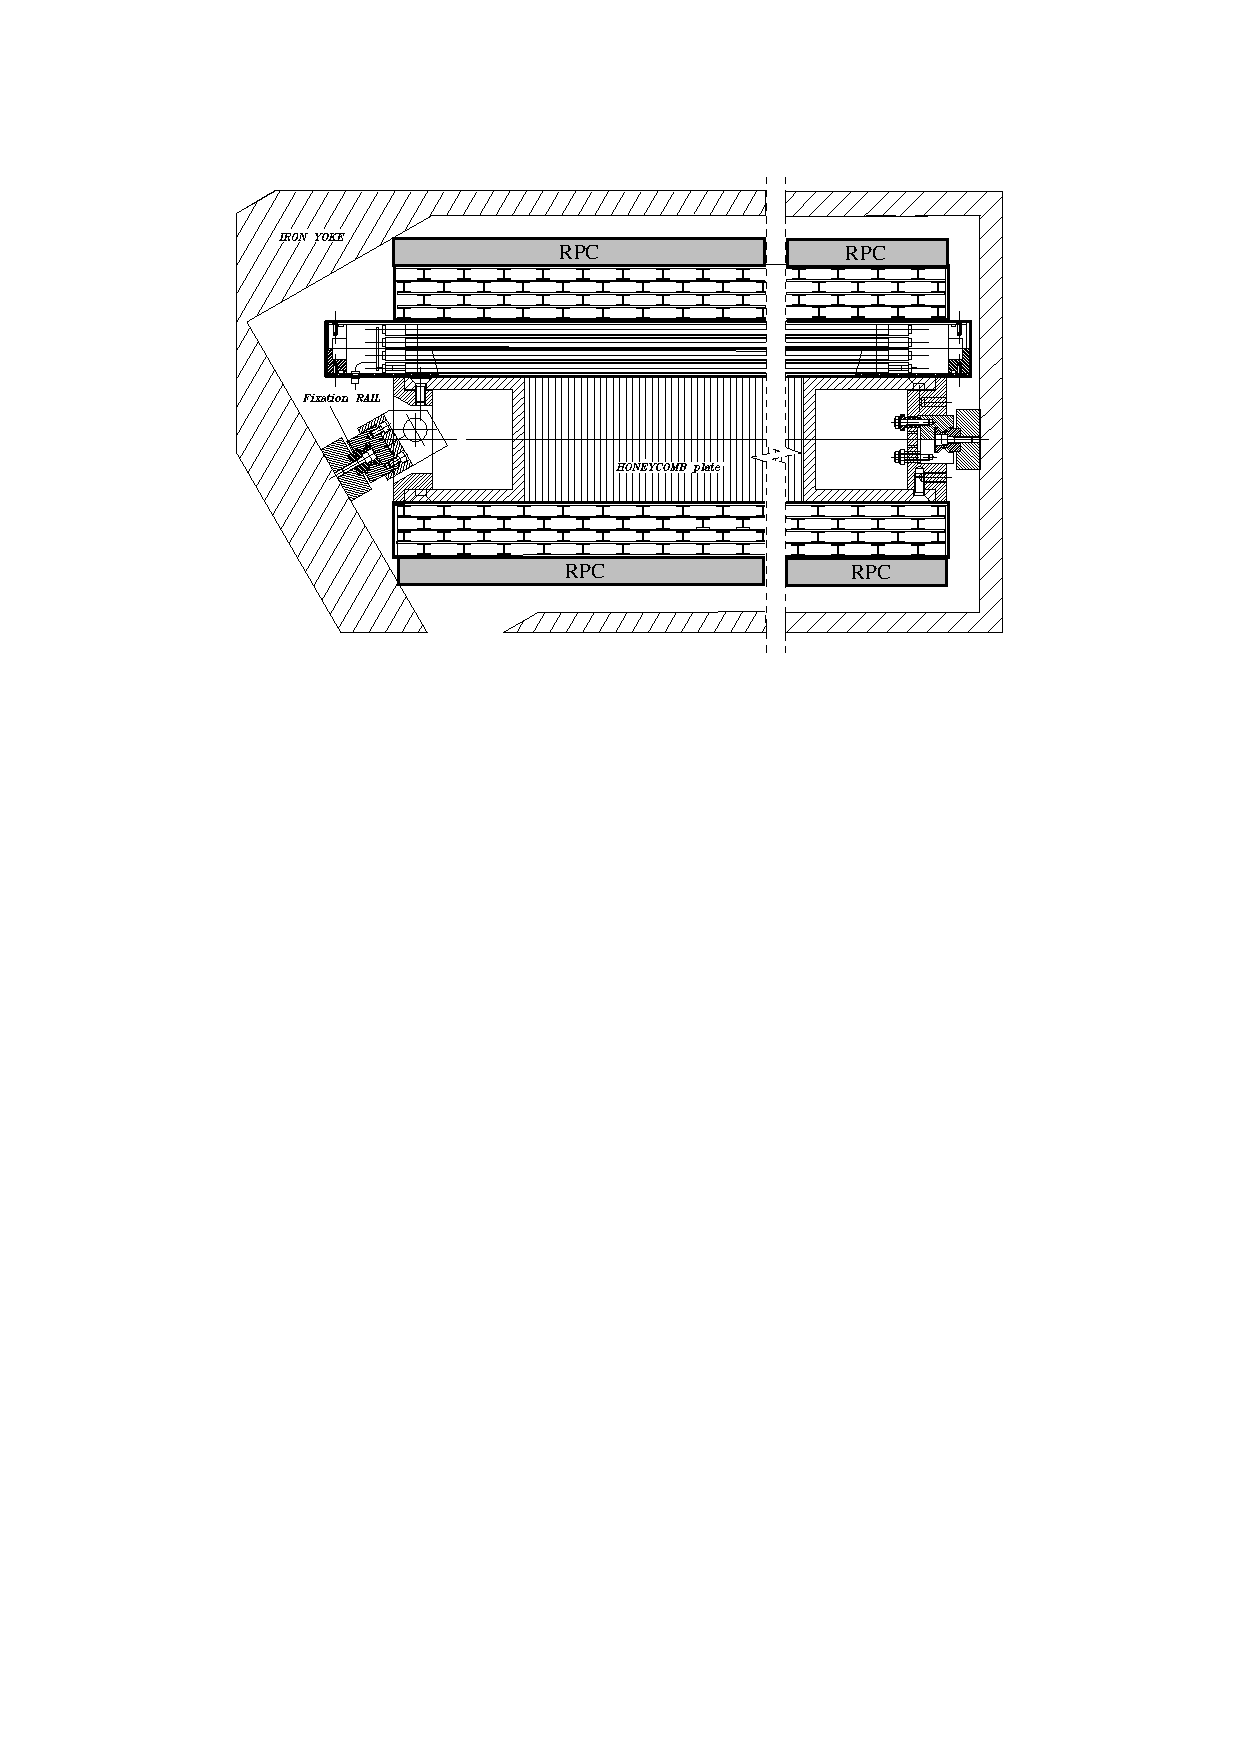
\includegraphics[width=0.80\textwidth]{figures/cms_muonsystem_honeycomb.pdf}
\caption{Chambers of the CMS DT system including the honeycomb support. From \cite{Chatrchyan:2008aa}.}
\label{fig:dt_chambers}
\end{figure}

\begin{figure}[hbtp]
\centering
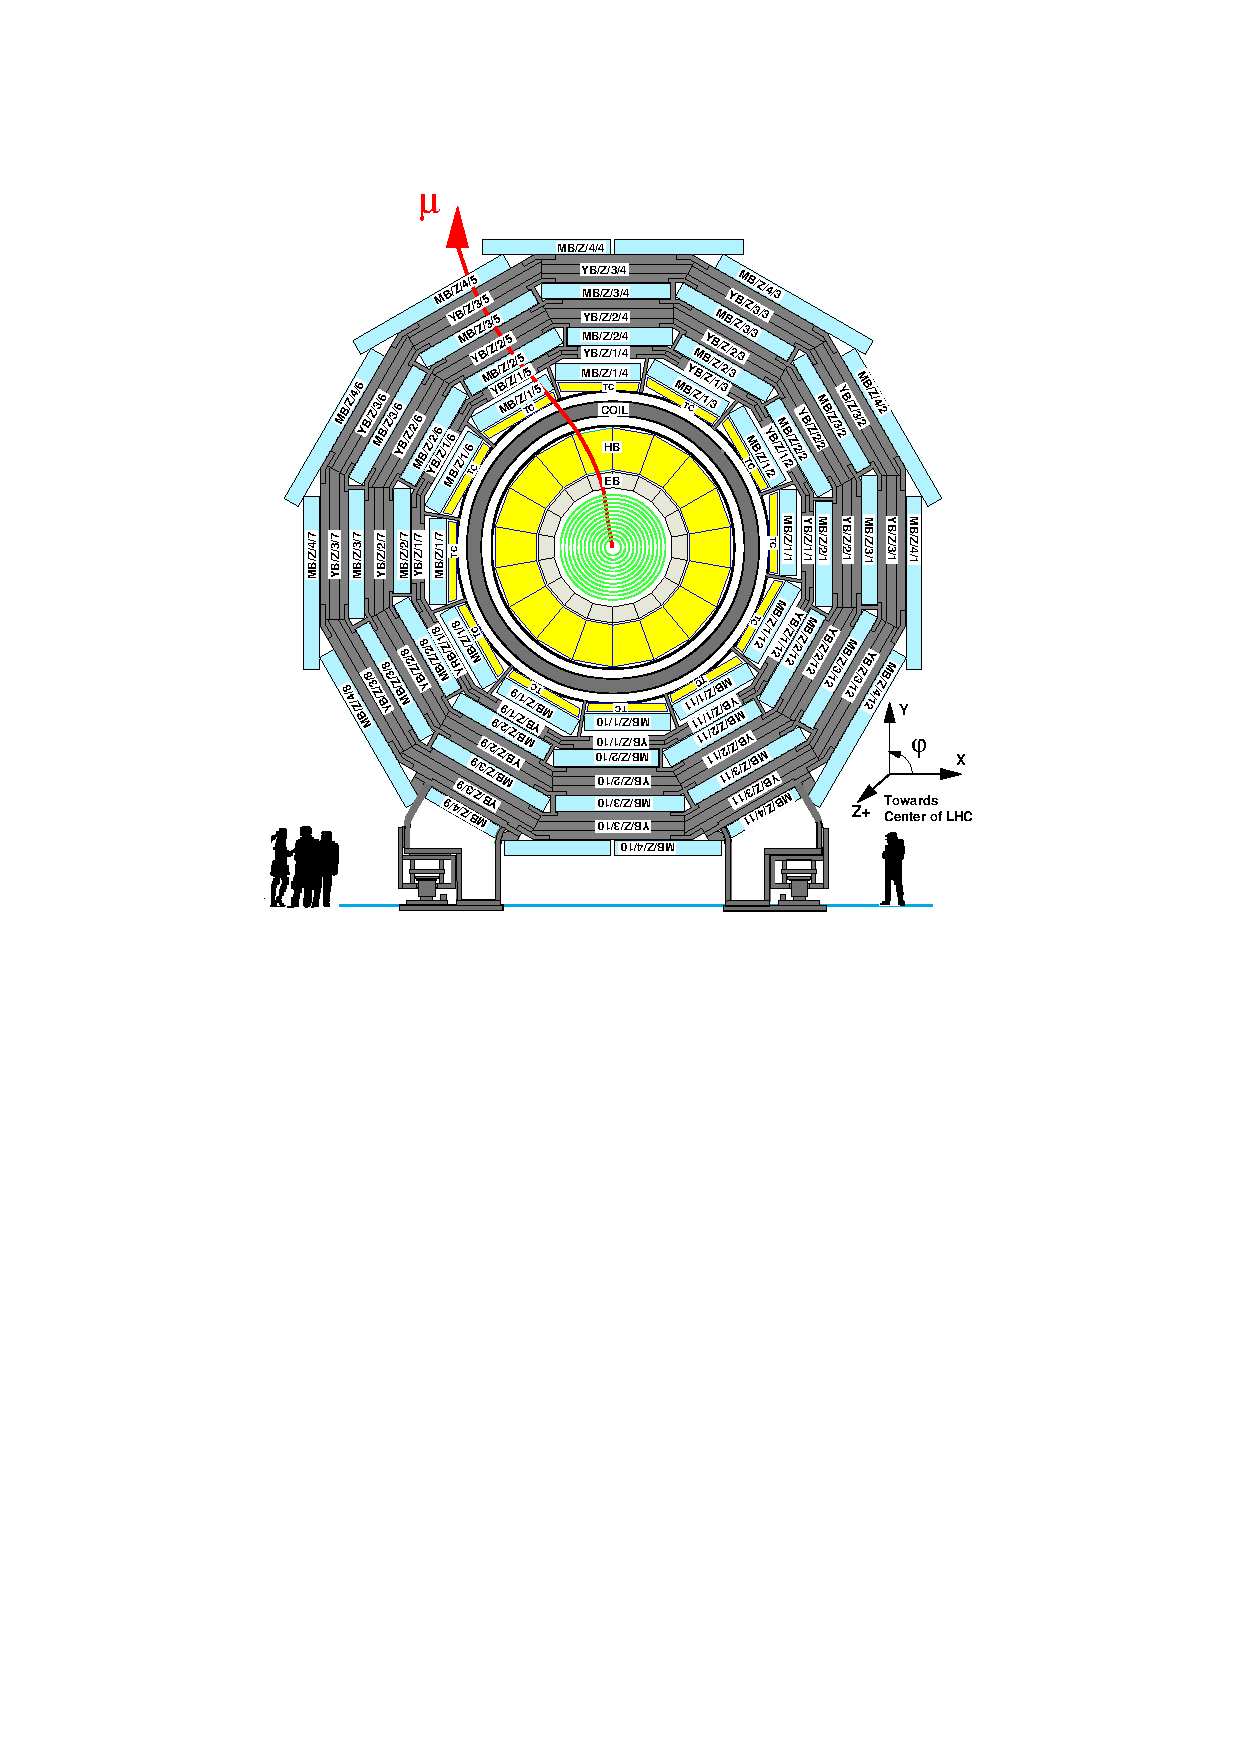
\includegraphics[width=0.8\textwidth]{figures/cms_drifttubes_slice.pdf}
\caption{ Layout of the CMS barrel muon DT chambers in one of the 5 wheels. From \cite{Chatrchyan:2008aa}.}
\label{fig:dt_barrel}
\end{figure}

\subsubsection{Cathode strip chambers}
The CSCs cover the pseudorapidity region $0.9<|\eta|<2.4$.
There are 4 stations of CSCs in each endcap.
The chambers are perpendicular to the beamline and interspersed between the magnetic flux return plates.
The cathode strips point radially outward from the beamline and provide a precision measurement in the $r-\phi$ bending plane.

The CSCs are multiwire proportional chambers comprised of 6 anode wire planes interleaved
among 7 cathode panels. Wires run azimuthally and define a track's radial coordinate.
Strips are milled on cathode panels and run lengthwise at constant $\Delta\phi$ width. 
The muon coordinate along the wires is obtained by interpolating between charges induced on strips.
The largest chambers, ME2/2 and ME3/2, are about $3.4 \times 1.5$ m\textsuperscript{2} in size.
The overall area covered by the sensitive planes of all chambers is about 5,000 m\textsuperscript{2},
the gas volume is over 50 m\textsuperscript{3}, and there are about 2 million wires.
There are about 9000 high-voltage channels in the system, 
about 220,000 cathode strip read-out channels with 12-bit signal digitization,
and about 180 000 anode wire read-out channels.

An avalanche on a wire induces charge on a cathode plane.
The charge shape can be approximately parameterized by the Gatti function;
see Equation 15 in Ref.~\cite{GATTI197983}.
Given the CSC geometry, most of the induced charge is shared among three or four strips.
A strip signal waveform is sampled and digitized every 50 ns.
The overal pulse duration is about 300 ns.
The charge cluster is fit to obtain the spatial coordinate, time, and cluster charge.
Using this method, the spatial resolution for a 6-plane chamber is 80 $\mathrm{\mu m}$.

\begin{figure}[hbtp]
\centering
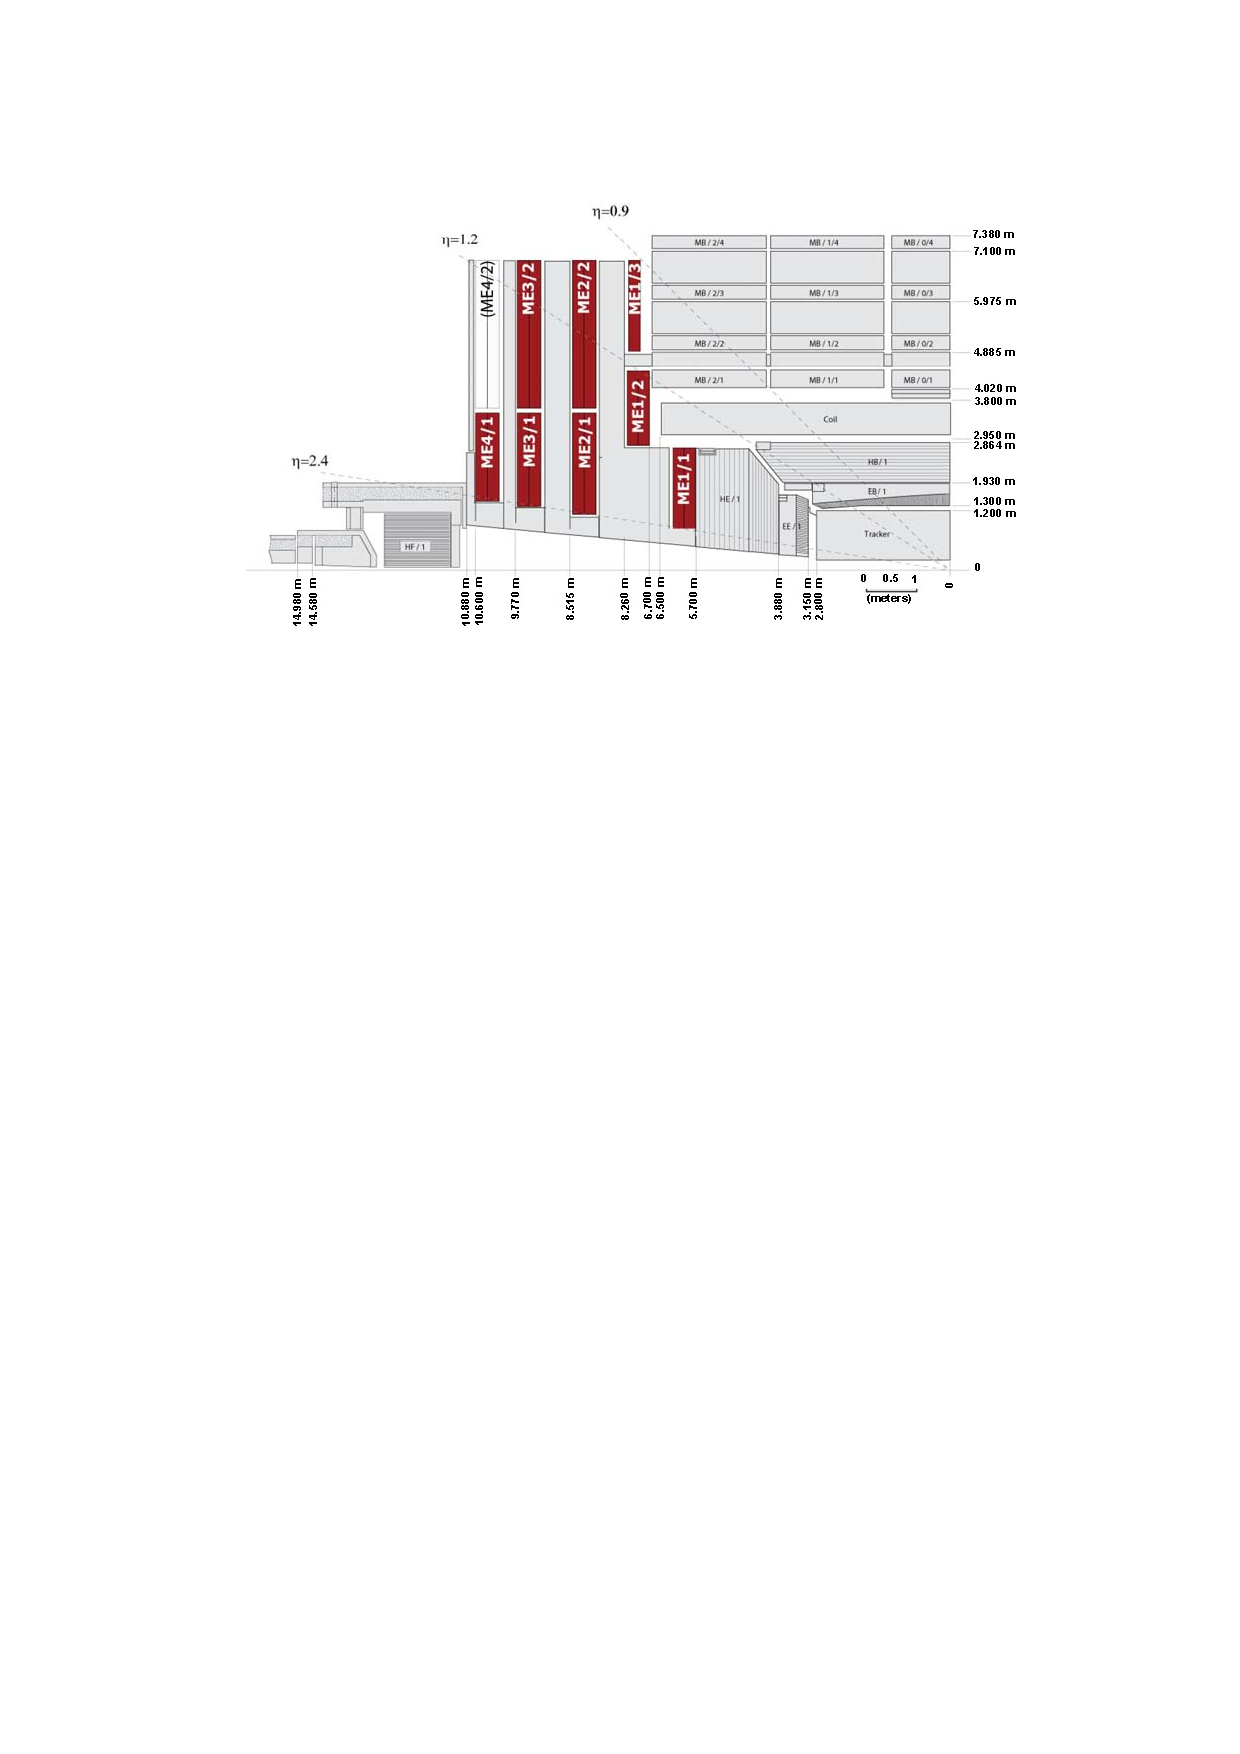
\includegraphics[width=0.8\textwidth]{figures/cms_quarter_csc_red.pdf}
\caption{
Quarter-view of the CMS detector. Cathode strip chambers of the Endcap Muon
system are highlighted.
From \cite{Chatrchyan:2008aa}.
}
\label{fig:cms_quarter_csc_red}
\end{figure}

\begin{figure}[hbtp]
\centering
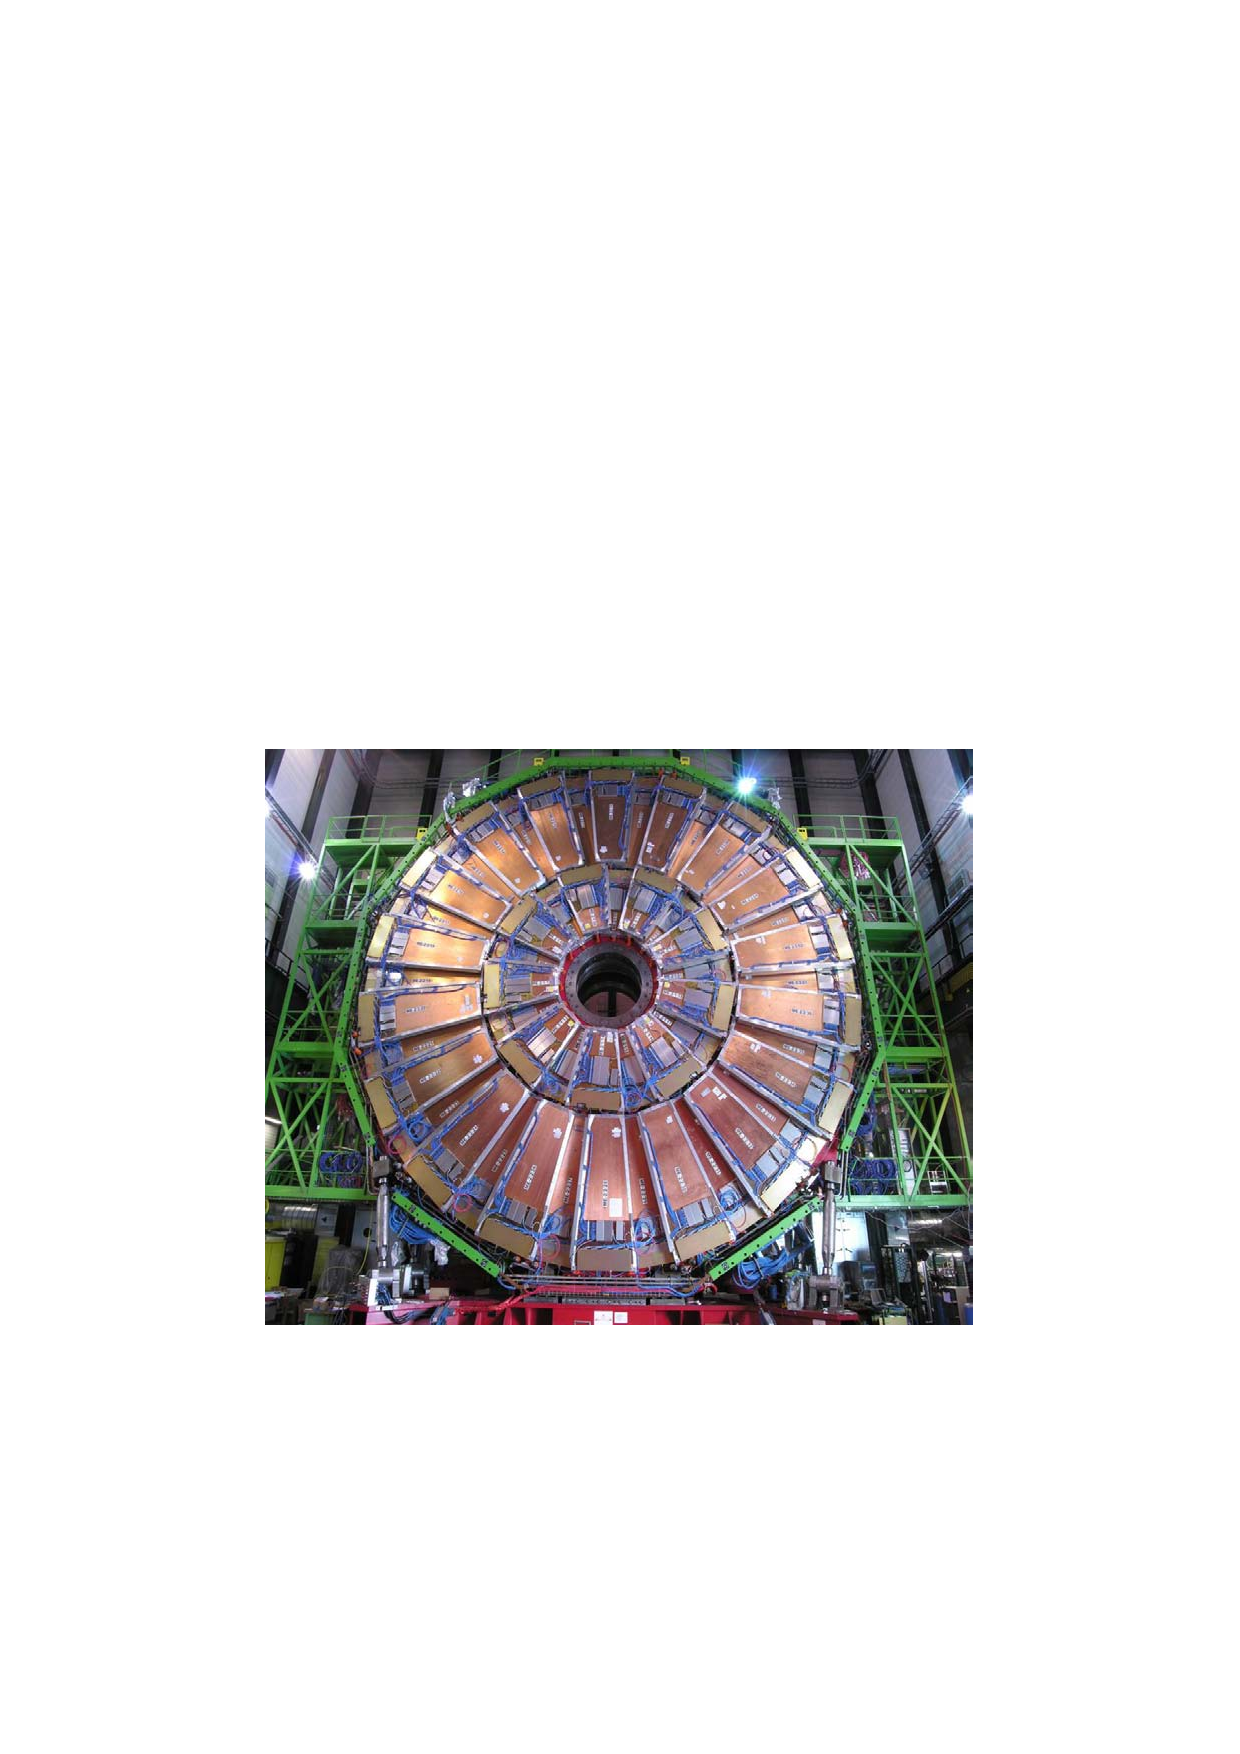
\includegraphics[width=0.8\textwidth]{figures/cms_cscs_me2.pdf}
\caption{
The ME2 station of CSCs. The outer ring consists of 36 ME2/2 chambers, each
spanning 10\degree in $\phi$, and the inner ring of eighteen 20\degree ME2/1 chambers.
The chambers overlap to provide contiguous coverage in $\phi$.
From \cite{Chatrchyan:2008aa}.
}
\label{fig:cms_cscs_me2}
\end{figure}

\subsubsection{Resistive plate chambers}

The RPCs are gaseous parallel-plate detectors with adequate spatial resolution and scintillator-level time resolution.
They are much faster than the 25 ns proton bunch crossing period at the LHC.
Using the RPC information, there is no ambiguity in the association of muon tracks and bunch crossings.

The CMS RPC basic double-gap module consists of two gaps operated in avalanche mode with common
pickup readout strips between them.
The total induced signal is the sum of the two single-gap signals.
Thus, the single-gaps can operate at a lower voltage gap,
with better effective efficiency than a single gap.

In the barrel iron return yoke, the RPC chambers form 6 coaxial sensitive cylinders
that are approximated with concentric dodecagon arrays arranged into 4 stations. See Figure~\ref{fig:cms_rpc_barrel}.

\begin{figure}[hbtp]
\centering
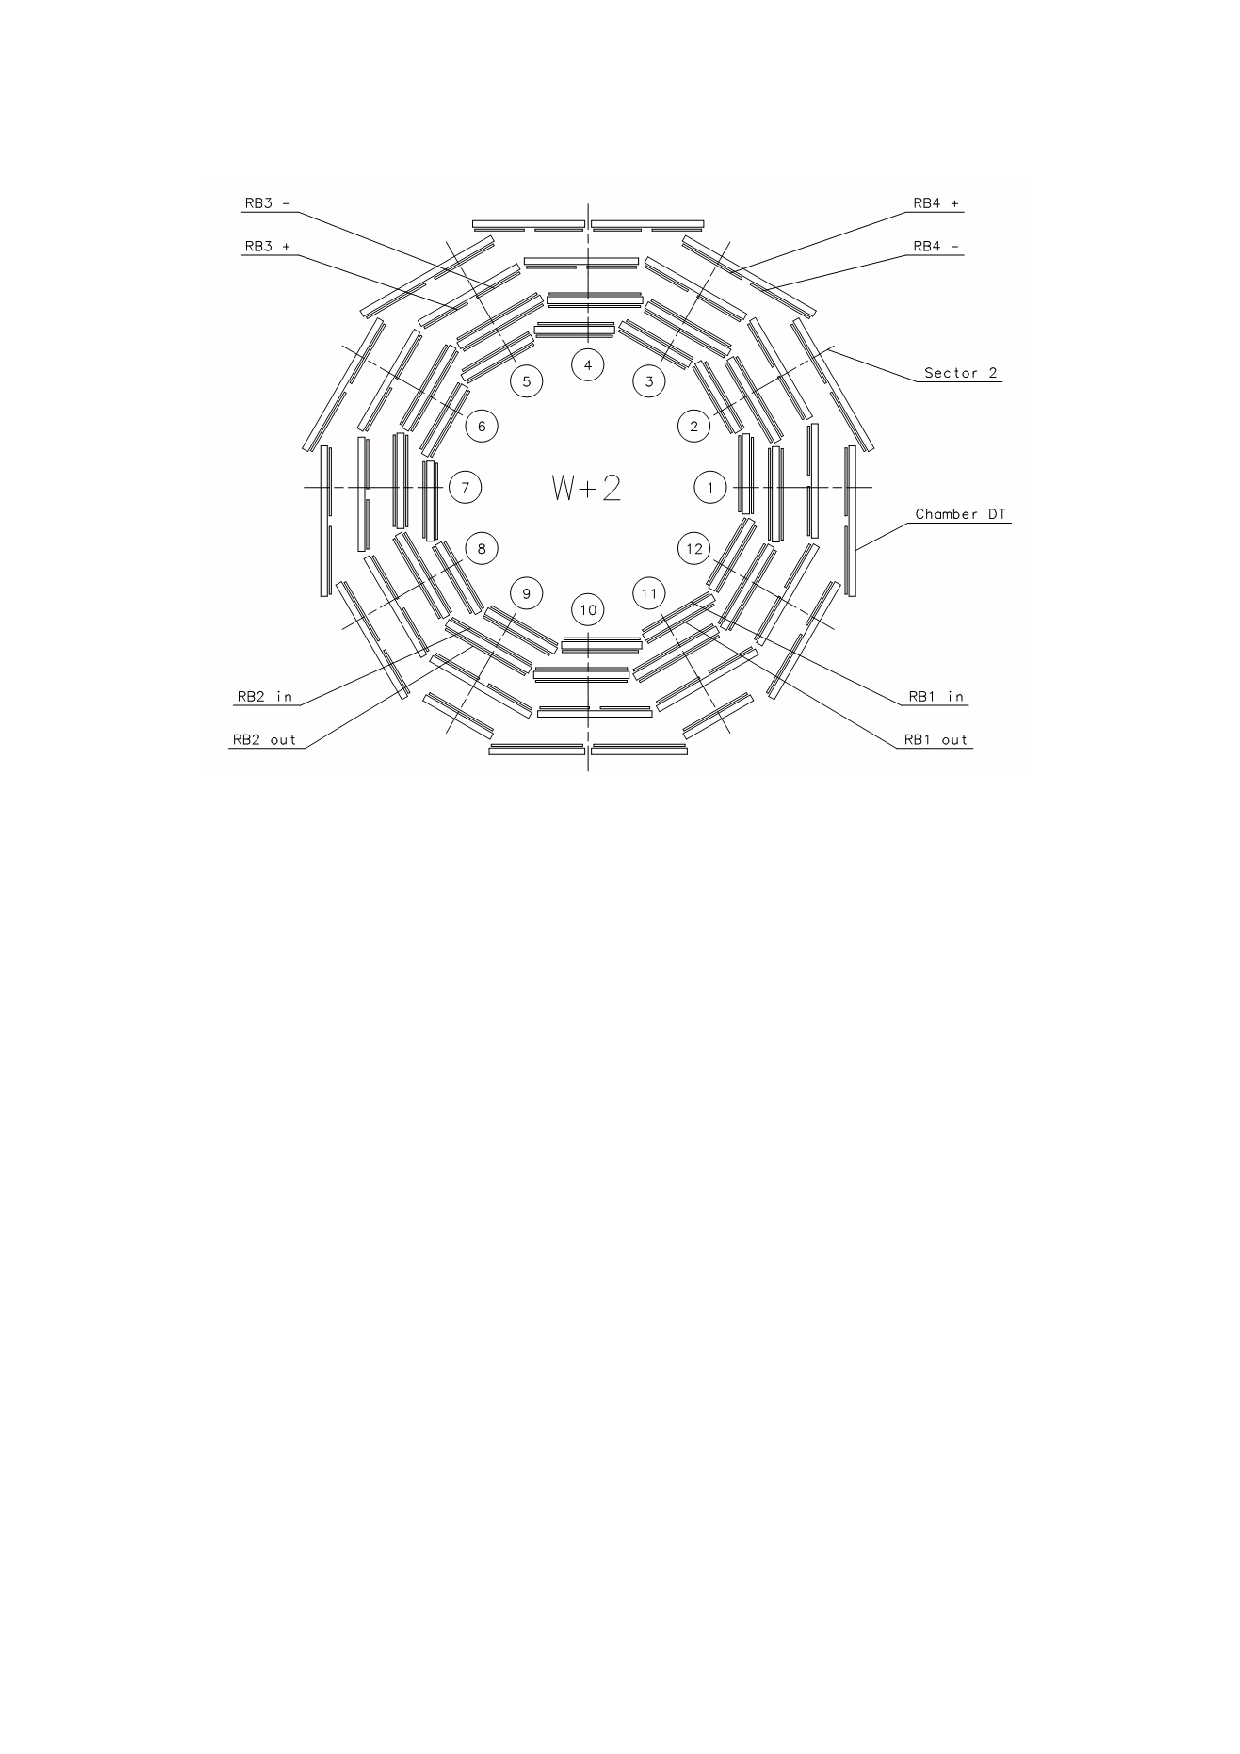
\includegraphics[width=0.8\textwidth]{figures/cms_rpc_barrel.pdf}
\caption{
Schematic layout of one of the 5 RPC barrel wheels. Each wheel is divided into 12 sectors.
From \cite{Chatrchyan:2008aa}.
}
\label{fig:cms_rpc_barrel}
\end{figure}
\clearpage

\subsection{Trigger system}
Triggering algorithms decide which data are recorded in the experiment.
They are implemented in two stages via a combination of hardware and software.

\subsubsection{Level-1 trigger}
The trigger decision process begins with the Level-1 Trigger (L1T) \cite{Khachatryan:2016bia}.  
The hardware implementation of the Level-1 Trigger is in the form of application-specific
integrated circuits (ASICs), field-programmable gate arrays (FPGAs), 
programmable logic devices (PLDs), and random access memory used for memory look-up tables (LUTs).
The FPGAs and LUTs may be reprogrammed, allowing for the algorithms to be revised.

The Level-1 Trigger is subject to a large data flow carried on optical fibers, 
copper cables, and backplanes within hardware crates. 
The data is transmitted in parallel at frequencies which are integer multiples of 40 MHz.
Data events passing the Level-1 Trigger are then transmitted to the so-called ``high-level trigger,'' described next.

\subsubsection{High-Level Trigger}
Data events accepted by the Level-1 Trigger are next processed by the High-Level Trigger (HLT).
Unlike the L1T's readout boards, the HLT is implemented on a commercial Linux computing cluster
called the File-based Filter Farm (F\textsuperscript{3}). There are three types of computing units in the F\textsuperscript{3}:
\begin{itemize}
\item The Readout Units take the information from the readout boards and assemble event fragments from a given detector partition.
\item The Builder Units take the event fragments and assemble full events. The full events are buffered here during the next step.
\item The Filter Units apply the final event selection of the HLT algorithms.
\end{itemize}
The HLT algorithms running on the FUs operate on full-granularity event data
from all subdetector systems. They accept between 1-10\% of events accepted by the L1T.
The algorithms make use of the CMS offline reconstruction framework called CMSSW.

\subsection{Offline world}
Events accepted by the HLT are merged into larger agglomerate files which are stored
locally in a Lustre parallel distributed file system.
Then, they are transferred from the ``online'' CMS experimental site to the
``offline'' CERN Tier-0 computing center at the main CERN campus in Meyrin for processing.
This transfer system is a multithreaded software,
optimized to handle rates of several gigabytes per second during data taking.
Finally, data are distributed worldwide from Tier-0 to the global CMS computing grid for physics studies.
